\documentclass[times, utf8, zavrsni, numeric]{fer}
\usepackage{booktabs}
\usepackage{url}
\usepackage{algorithmic}
\usepackage{algorithm}
\usepackage{multirow}
\usepackage{numprint}
\usepackage{placeins}
\usepackage{afterpage}

\makeatletter
\renewcommand{\ALG@name}{Pseudokod}
\newcommand{\norm}[1]{\lVert#1\rVert}
\newcommand*\bigcdot{\mathpalette\bigcdot@{.5}}
\newcommand*\bigcdot@[2]{\mathbin{\vcenter{\hbox{\scalebox{#2}{$\m@th#1\bullet$}}}}}
\makeatother

\begin{document}

% TODO: Navedite broj rada.
\thesisnumber{5671}

% TODO: Navedite naslov rada.
\title{Postupci za višekriterijsku i mnogokriterijsku optimizaciju}

% TODO: Navedite vaše ime i prezime.
\author{Luka Banović}

\maketitle

% Ispis stranice s napomenom o umetanju izvornika rada. Uklonite naredbu \izvornik ako želite izbaciti tu stranicu.
\izvornik

% Dodavanje zahvale ili prazne stranice. Ako ne želite dodati zahvalu, naredbu ostavite radi prazne stranice.
\zahvala{}

\tableofcontents

\chapter{Uvod}
Višekriterijska optimizacija ima primjenu u svakom problemu u kojem je potrebno pronaći optimalni kompromis između više različitih kriterija, gdje su kriteriji nužno međusobno suprotstavljeni, npr. pri dizajnu automobila to su brzina, sigurnost i potrošnja goriva. Kada kriteriji ne bi bili suprotstavljeni, tada kompromis ne bi bilo potrebno postići jer je moguće dobiti ekstremne vrijednosti za svaki kriteriju odjednom. Kada se poveća broj kriterija, tada možemo govoriti o mnogokriterijskoj optimizaciji, ali u ovom radu se izraz višekriterijska optimizacija koristi u oba slučaja. U nastavku, definira se problem višekriterijske optimizacije, izlaže se njezin dosadašnji razvoj te pobliže opisuje nekoliko odabranih algoritama kojima se ona provodi. Na kraju se algoritmi uspoređuju na odabranom skupu ispitnih primjera.

\section{Problem višekriterijske optimizacije}
\label{sec:kriterij}
Prema \citep{pioa2013}, definicija problema višekriterijske optimizacije jest:
\begin{align*}
\mbox{Optimiziraj } &f_m(\vec{x}),\quad m = 1,\dots,M \\
\mbox{uz ograničenja } &g_j(\vec{x}) \geq 0, \quad j = 1,\dots,J \\
&h_k(\vec{x}) = 0, \quad k = 1,\dots,K \\
&{x_i}^L \leq x_i \leq {x_i}^U, \quad i = 1,\dots,n
\end{align*}
Ovdje je rješenje $\vec{x} = \{x_1, x_2, \dots, x_n\}$ vektor decizijskih varijabli \engl{decision variables}, a prvi i drugi skup nejednakosti definiraju ograničenja koja moraju ispunjavati sva prihvatljiva rješenja \engl{feasible solutions}, dok treći skup nejednakosti postavlja granice vrijednosti koje decizijske varijable smiju poprimiti. Ovi skupovi određuju prostor prihvatljivih rješenja, gdje je jedno rješenje točka u tom prostoru. \\
Budući da se problem minimizacije neke funkcije $g$ može svesti na problem maksimizacije funkcije $-g$, 
vrlo je česta formulacija problema višekriterijske optimizacije minimizacija, odnosno maksimizacija svih
ciljnih funkcija \engl{objective function}. Međutim, neki od algoritama korištenih u ovom radu vrlo su 
osjetljivi na takvu promjenu, o čemu će više riječi biti u nastavku.
\section{Pareto optimalnost}
Kod jednokriterijske optimizacije vrlo je jednostavno odrediti koje je rješenje najbolje: svakom se rješenju pridijeli iznos određen funkcijom dobrote \engl{fitness function} te se odabere rješenje kojemu je pridijeljen najveći, odnosno najmanji iznos funkcije dobrote --- ovisno o tome radi li se o maksimizaciji ili minimizaciji.\\
Međutim, takav pristup nije moguć kod višekriterijske optimizacije jer ne postoji jedna funkcija koju se pokušava optimizirati, nego veći broj njih --- umjesto skalarne vrijednosti, dobrota rješenja je prikazana pomoću vektora. Komponente tog vektora su vrijednosti ciljnih funkcija (funkcija koje želimo optimirati). Tako kod višekriterijske optimizacije govorimo o dva prostora: prostoru decizijskih varijabli \engl{decision space} i prostoru ciljnih funkcija \engl{objective space}. \\
Uvođenjem većeg broja ciljnih funkcija jednostavnost usporedbe rješenja nestaje. Primjerice, promotrimo dva rješenja čiji su vektori ciljnih funkcija $\vec{a} = (3,4)$ i $\vec{b} = (2,3)$ te pretpostavimo da nam je cilj maksimizirati obje ciljne funkcije. Prvo je rješenje bolje po prvoj ciljnoj funkciji, a drugo po drugoj, te ne možemo odrediti koje je od njih, općenito gledano, bolje --- nad rješenjima nije definiran potpuni uređaj. Jedno od prvih rješenja ovakvog problema je svesti problem višekriterijske optimizacije na jednokriterijsku dodijelivši težinu svakoj ciljnoj funkciji te izračunavši  
\begin{align*}
f = \sum_{i=1}^M w_i \cdot y_i.
\end{align*}
Ovdje je $M$ broj ciljnih funkcija, $w_i$ težina $i$-te ciljne funkcije, a $y_i$ vrijednost $i$-te ciljne funkcije. \\
Osim toga, jedno od mogućih rješenja je sortiranje ciljnih funkcija po prioritetu od najvažnije do najmanje važne. Tada se dva rješenja, $\vec{x}^{(1)}$ s pridruženim vektorom ciljnih funkcija $\vec{y}^{(1)} = \{y_1^{(1)}, \dots, y_M^{(1)}\}$ i $\vec{x}^{(2)}$ kojemu je pridružen vektor $\vec{y}^{(2)}~ = ~\{y_1^{(2)}, \dots, y_M^{(2)}\}$, uspoređuju na sljedeći način:
\begin{itemize}
\item jednaka su ako $\forall i \in \{1,\dots, M\}$ vrijedi $\vec{y_i}^{(1)} = \vec{y_i}^{(2)}$,
\item rješenje $\vec{x}^{(1)}$ je bolje od rješenja $\vec{x}^{(2)}$ ako $\exists j \in \{1,\dots,M\}, \forall i \in \{1,\dots,M\} \land i < j$ vrijedi $y_i^{(1)} = y_i^{(2)}$ i $y_j^{(1)}$ je bolje od $y_j^{(2)}$,
\item rješenje $\vec{x}^{(1)}$ je lošije od rješenja $\vec{x}^{(2)}$ ako $\exists j \in \{1,\dots,M\}, \forall i \in \{1,\dots,M\} \land i < j$ vrijedi $y_i^{(1)} = y_i^{(2)}$ i $y_j^{(1)}$ je lošije od $y_j^{(2)}$.
\end{itemize}
Nakon što se problem višekriterijske optimizacije na ovaj način svede na jednu funkciju koju je potrebno optimizirati, moguće je pronaći optimalno rješenje uobičajenim algoritmima za jednokriterijsku optimizaciju.\\
Najveća mana navedenih pristupa je što pronalaze samo jedno optimalno rješenje. Ako iz nekog razloga promijenimo prioritete ciljnim funkcijama ili njihove težine, moramo ponoviti postupak optimizacije. Drugim riječima, svođenje problema višekriterijske optimizacije na jednokriterijsku od korisnika zahtijeva opis njegovih prioriteta prije same optimizacije.  \\
S druge strane, pristup koji je najbolje prihvaćen u području višekriterijske optimizacije, jest uvođenje relacije dominacije. Kažemo da rješenje $\vec{x}^{(1)}$ dominira nad rješenjem $\vec{x}^{(2)}$ ako rješenje $\vec{x}^{(1)}$ nije gore od rješenja $\vec{x}^{(2)}$ ni u jednoj ciljnoj funkciji i postoji barem jedna ciljna funkcija u kojoj je rješenje $\vec{x}^{(1)}$ strogo bolje od rješenja $\vec{x}^{(2)}$. Relacija dominacije nije simetrična ni refleksivna, ali jest tranzitivna. Sada se i cilj optimizacije mijenja: umjesto pronalaženja jednog optimalnog rješenja, želimo pronaći podskup skupa rješenja koji čine rješenja nad kojima nijedno drugo rješenje u prostoru ne dominira. Nedominirani podskup skupa svih prihvatljivih rješenja naziva se Pareto optimalni skup, a skup pripadnih vektora u prostoru ciljnih funkcija naziva se Pareto fronta. Treba primijetiti da su algoritmi koji nastoje odrediti Pareto optimalan skup potpuno neovisni o korisniku --- korisnik samo treba odabrati rješenje iz skupa koje odgovara njegovim potrebama.
\section{Pregled područja}
Jedan od najranijih pokušaja rješavanja problema višekriterijske optimizacije je algoritam VEGA, primjena genetskog algoritma u višekriterijskoj optimizaciji \citep{vega}, temeljen na usporedbi vektora dobrote. No, kako je pokazivao pristranost u odabiru rješenja, nije ušao u širu uporabu. Kasnije su predloženi različiti algoritmi koji su za namjeru imali eliminaciju ove pristranosti: MOGA \citep{moga}, NPGA \citep{npga} i NSGA \citep{nsga}. Daljnji napredak je ostvaren kad je prepoznato da prenošenje najboljih rješenja između generacija daje bolje rezultate. Tako je predložen SPEA \citep{spea} koji je rezultatima ubrzo nadmašio postojeće algoritme. Međutim, ubrzo su novi algoritmi kao NSGA-II \citep{nsga2} i PESA \citep{pesa} proizveli bolje rezultate nego SPEA, te su ga autori poboljšali, predloživši SPEA2 \citep{spea2}. Kako su tada postojeći algoritmi davali vrlo dobre rezultate za probleme s manjim brojem ciljnih funkcija, a iznimno loše ukoliko bi se taj broj povećao, pojavila se potreba za algoritmima koji će rješavati veće probleme. S tim u vidu nastali su NSGA-III \citep{nsga3} i MOEA/D \citep{moead}, a u ovom se smjeru nastavlja sadašnji razvoj ovog područja.

\chapter{Algoritmi}
U sklopu ovog rada, implementirani su sljedeći algoritmi: NSGA, NSGA-II, \mbox{NSGA-III}, SPEA2 te dvije varijante MOEA/D algoritma. Svaki od njih bit će pobliže objašnjen u nastavku. Budući da se svi navedeni algoritmi temelje na genetskom algoritmu (za jednokriterijsku optimizaciju), moguće je objasniti njihovu zajedničku osnovnu ideju.\\
Kroz više generacija, tj. iteracija algoritma, čuva se skup rješenja određene veličine. Takav skup se naziva populacija, a elementi skupa su jedinke. Tijekom jedne generacije, pomoću operatora selekcije \engl{selection}, odabiru se jedinke čiji će potomci biti jedinke iduće populacije. Selekcija mora biti takva da osigura najveću vjerojatnost izbora jedinki koje su najbolje. Potomci se zatim stvaraju operatorom križanja \engl{crossover}. Postoji više različitih načina križanja, ali zajedničko im je da se ono odvija u prostoru decizijskih varijabli, a poželjno im je svojstvo da dobiveni potomci budu blizu roditeljima, tj. da preuzmu neke od karakteristika svojih roditelja. I na kraju, operatorom mutacije \engl{mutation} mutira se svaki dobiveni potomak. Cilj mutacije je uvesti raznolikost u populaciju te omogućiti istraživanje različitih dijelova prostora prihvatljivih rješenja. Mutacija se ne mora uvijek dogoditi --- prije pokretanja algoritma postavlja se vjerojatnost mutacije (vjerojatnost da će mutirati jedna decizijska varijabla promatranog rješenja). I na kraju, populacija dobivena ovim postupkom postaje roditeljska populacija u sljedećoj generaciji.\\
Potrebno je napomenuti da se operatori križanja i mutacije nimalo ili vrlo malo razlikuju između različitih algoritama. Najveća razlika se pojavljuje u operatoru selekcije, tj. osiguravanju raznolikosti rješenja.

\section{NSGA}
\subsection{Uvod}
Algoritam NSGA (Nondominated Sorting Genetic Algorithm) prvi je put predstavljen u radu Srinivasa i Deba \citep{nsga}. Osnovna ideja je generacijski genetski algoritam koji je prilagođen višekriterijskoj optimizaciji zahvaljujući drukčijoj selekciji rješenja temeljenoj na nedominiranom sortiranju. 
\subsection{Opis algoritma}
Jedna generacija algoritma započinje evaluacijom svih rješenja u populaciji (određivanjem vektora ciljnih funkcija za svako rješenje). Rješenja u trenutnoj populaciji se zatim sortiraju po nedominiranosti u fronte: u prvoj se fronti nalaze nedominirana rješenja, u drugoj rješenja nad kojima dominiraju samo rješenja iz prve fronte itd. Pseudokod \ref{algo:non-dom} prikazuje implementaciju procedure za nedominirano sortiranje. Sortiranje se odvija u dvije faze. U prvoj se fazi za svako rješenje određuje skup rješenja nad kojima ono dominira ($S_i$) te broj rješenja ($\eta_i$) koje dominiraju nad njim. Sva se rješenja za koja je $\eta_i = 0$ zatim dodaju u prvu frontu. U drugoj fazi određuju se iduće fronte na sljedeći način: za svako rješenje $x_i$ iz trenutne fronte $F_k$ iteriramo kroz skup rješenja nad kojima ono dominira. Za svako rješenje $x_j$ koje nađemo tamo smanjimo njegov brojač $\eta_i$ za 1. Ako tada brojač padne na 0, to rješenje postaje dio iduće fronte $F_{k+1}$. Postupak se ponavlja dok god trenutna populacija nije prazna.\\
\begin{algorithm}
\caption{Nedominirano sortiranje}
\label{algo:non-dom}
\begin{algorithmic}
\STATE{\textbf{Input:} $P$ -- populacija koju je potrebno sortirati.}
\STATE{\textbf{Output:} $\{F_1, \dots, F_m\}$ -- skup fronti na koje je populacija podijeljena}
\STATE $F_1 = \emptyset$
\FOR{$\vec{x}^{(i)} \in P$}
\STATE{$\eta_i = 0, S_i = \emptyset$}
\FOR{$\vec{x}^{(j)} \in P, \vec{x}^{(j)} \neq \vec{x}^{(i)}$}
\IF{$\vec{x}^{(i)}$ dominira nad $\vec{x}^{(j)}$}
\STATE $S_i = S_i \cup \{\vec{x}^{(j)}\}$
\ELSIF{$\vec{x}^{(j)}$ dominira nad $\vec{x}^{(i)}$}
\STATE{$\eta_i = \eta_i + 1$}
\ENDIF
\ENDFOR
\IF{$\eta_i = 0$}
\STATE $F_1 = F_1 \cup \{\vec{x}^{(i)}\}$
\ENDIF
\ENDFOR
\STATE{$k = 1$}
\WHILE{$F_k \neq \emptyset$}
\STATE $Q = \emptyset$
\FOR{$\vec{x}^{(i)} \in F_k$}
\FOR{$\vec{x}^{(j)} \in S_i$}
\STATE {$\eta_j = \eta_j - 1$}
\IF{$\eta_j = 0$}
\STATE{$Q = Q \cup \{\vec{x}^{(j)}\}$}
\ENDIF
\ENDFOR
\ENDFOR
\STATE{$k = k + 1, F_k = Q$}
\ENDWHILE
\end{algorithmic}
\end{algorithm}
Nakon što su rješenja iz populacije sortirana, pridjeljuje im se dobrota ovisno o fronti u kojoj se nalaze i udaljenosti od ostalih rješenja. Ukratko, ideja je da rješenja koja se nalaze u prvoj fronti i koja unutar nekog radijusa, određenog parametrom $\sigma_{share}$, dobiju puni iznos dobrote, dok se ostalim rješenjima taj iznos smanjuje. Udaljenost između rješenja se računa u prostoru rješenja izrazom:
\begin{align*}
d_{ij} = \sqrt{\sum_{k=1}^n\left(\frac{x_k^{(i)} - x_k^{(j)}}{x_k^{{max}} - x_k^{{min}}}\right)^2}
\end{align*}
Na temelju udaljenosti $d$ računa se vrijednost funkcije dijeljenja $\engl{sharing function}$:
\[
    sh(d)= 
\begin{cases}
    1 - \left(\frac{d}{\sigma_{share}}\right)^\alpha,& \text{za } d < \sigma_{share} \\
    0,              & \text{inače.}
\end{cases}
\]
Funkcija dijeljenja nam je potrebna da izračunamo gustoću niše \engl{niche density}, odnosno mjeru koja za pojedino rješenje opisuje koliko je rješenja u njegovoj okolini i koliko su ona blizu. Izraz za gustoću niše glasi:
\begin{align*}
nc_i = \sum_{j=1}^N sh(d_{ij})
\end{align*}
Sada napokon imamo sve što nam je potrebno da bismo za neko rješenje $\vec{x}$ iz populacije mogli izračunati dijeljenu dobrotu s kojim NSGA radi. Cijeli postupak je prikazan~pseudokodom~\ref{algo:nsga-fit}.\\

\begin{algorithm}
\caption{Dodjela dobrote kod NSGA}
\label{algo:nsga-fit}
\begin{algorithmic}
\STATE{\textbf{Input:} $\{Q_1, \dots, Q_m\}$ -- sortirana rješenja, $\sigma_{share}$.}
\STATE{$\epsilon = \mbox{mala pozitivna konstanta}$, $F_{min} = N + \epsilon$}
\FOR{$j=1; j<=m; j = j+1$}
\FOR{$q \in Q_j$}
\STATE{$F_j^{(q)} = F_{min} - \epsilon$}
\STATE{Odredi gustoću niše $nc_q$ uračunavajući samo rješenja iz $Q_j$}
\STATE{Odredi dijeljenu dobrotu $F_j^{'(q)} = \frac{F_j^{(q)}}{nc_q}$}
\ENDFOR
\STATE{$F_{min} = min(F_j^{'(q)}:q\in Q_j)$}
\ENDFOR
\end{algorithmic}
\end{algorithm}

Pomoću dodijeljene dobrote sada možemo stvoriti novu populaciju pomoću operatora selekcije, križanja i mutacije, čime završavamo jednu generaciju. Opisani postupak je prikazan pseudokodom \ref{algo:nsga-one-gen}. Treba primijetiti da algoritam nije elitistički, odnosno ne čuva najbolja rješenja između generacija. Nadalje, zbog načina na koji se dodjeljuje dobrota jedinkama, kod NSGA je potrebno koristiti neku od inačica proporcionalne selekcije \engl{Roulette-wheel selection}. Kod proporcionalne selekcije, vjerojatnost izbora pojedine jedinke proporcionalna je njezinoj dobroti. Međutim, da bi ispravno radila, potrebno je osigurati da su sve dodijeljene dobrote nenegativne, a suma im mora biti pozitivna.\\

\begin{algorithm}
\caption{Jedna generacija NSGA}
\label{algo:nsga-one-gen}
\begin{algorithmic}
\STATE{\textbf{Input:} $P$ -- Trenutna populacija.}
\STATE{Evaluiraj $P$}
\STATE{Sortiraj $P$ po nedominiranosti}
\STATE Dodijeli dobrotu rješenjima iz $P$
\STATE Stvori novu populaciju iz $P$ pomoću selekcije, križanja i mutacije
\end{algorithmic}
\end{algorithm}

\section{NSGA-II}
\subsection{Uvod}
NSGA-II nastavak je NSGA algoritma. Nastao je iz nastojanja da se riješe problemi zbog kojih je NSGA kritiziran \citep{nsga2}:
\begin{itemize}
\item manjak elitizma,
\item potreba za specificiranjem parametra $\sigma_{share}$.
\end{itemize}
Novosti koje NSGA-II donosi su nova vrsta operatora selekcije i smanjen broj potrebnih parametara, budući da izbacuje parametre potrebne za računanje gustoće niše. Umjesto toga, uz nedominirano sortiranje, predlaže se grupirajuća turnirska selekcija gdje je potrebno jedino odabrati veličinu turnira.
\subsection{Opis algoritma}
Algoritam započinje nedominiranim sortiranjem početne populacije $P_0$. Nakon toga, stvara se nova populacija djece $Q_0$ uporabom binarne turnirske selekcije te danih operatora križanja i mutacije. Zbog uvođenja elitizma, ostale se generacije razlikuju od početne. Prije nego opišemo glavnu petlju NSGA-II, ukratko ćemo se osvrnuti na turnirsku selekciju. $k$-turnirska selekcija je vrsta selekcije u kojoj se prvo iz populacije nasumično odabere $k$ jedinki i iz tog podskupa se odabere najbolja (pobjednik turnira) po nekoj usporedivoj mjeri dobrote. Primjerice, spomenuta binarna turnirska selekcija iz populacije nasumično odabire dvije jedinke, a pobjednik je turnira jedinka s manjim rangom, odnosno rednim brojem fronte u kojoj se nalaze nakon nedominiranog sortiranja.\\
Opišimo sada $t$-tu generaciju. Ona započinje formiranjem kombinirane populacije roditelja $P_t$ i djece $Q_t$, odnosno $R_t = P_t \cup Q_t$. Zatim se populacija $R_t$ nedominirano sortira. Buduća populacija roditelja $P_{t+1}$ stvara se od fronti $F_1,\dots, F_m$ na sljedeći način: redom, za svaku frontu iz skupa danih fronti, provjeravamo je li veličina trenutne fronte $F_i$ manja od broja potrebnih rješenja u $P_{t+1}$. Ako jest, sva rješenja iz dane fronte uključujemo u buduću populaciju roditelja. Postupak prestaje kada naiđemo na frontu za koju navedeni uvjet ne vrijedi. Označimo frontu za koju se to dogodi s $F_k$, a traženu veličinu populacije s $N$. Tada je potrebno još uključiti $K = N - \left\vert{P_{t+1}}\right\vert$ iz fronte $F_k$. Zato se prvo fronta $F_k$ silazno sortira po udaljenosti grupiranja \engl{crowding distance} te se onda $P_{t+1}$ popunjava sa $K$ rješenja s početka. Generacija završava stvaranjem nove populacije djece, $Q_{t+1}$, pomoću selekcije, križanja i mutacije. Cijeli postupak je opisan u pseudokodu \ref{algo:nsga2-one-gen}.

\begin{algorithm}
\caption{Jedna generacija NSGA-II}
\label{algo:nsga2-one-gen}
\begin{algorithmic}
\STATE{\textbf{Input:} $P_t$ -- trenutna populacija roditelja}
\STATE{\textbf{Input:} $Q_t$ -- trenutna populacija djece}
\STATE{$R_t = P_t \cup Q_t$}
\STATE{$F_1, dots, F_m =$ sortiraj $R_t$ po nedominiranosti}
\STATE{$P_{t+1} = \emptyset$, $i = 1$}
\WHILE{$\vert P_{t+1} \vert + \vert F_i \vert \leq N$}
\STATE{$P_{t+1} = P_{t + 1} \cup F_i$}
\STATE{$i = i+1$}
\ENDWHILE
\STATE{Sortiraj frontu $F_i$ po udaljenosti grupiranja}
\STATE{U $P_{t+1}$ dodaj $N - \vert P_{t+1} \vert$ prvih rješenja iz $F_i$}
\STATE{Stvori novu populaciju djece $Q_{t+1}$ iz $P_{t+1}$}
\end{algorithmic}
\end{algorithm}

Udaljenost grupiranja je veličina kojom se procjenjuje gustoća rješenja oko nekog rješenja u populaciji. Da bi se mogla odrediti, potrebno je rješenja uzlazno sortirati po svakoj ciljnoj funkciji. Za svaku ciljnu funkciju, rješenjima koja imaju najveću i najmanju vrijednost te funkcije dodjeljuje se beskonačna udaljenost grupiranja. Za sva rješenja kojima udaljenost grupiranja nije određena na ovaj način, udaljenost grupiranja se računa kao suma apsolutnih vrijednost normaliziranih razlika susjednih vrijednosti (pseudokod \ref{algo:nsga2-crowding-distance}).\\

\begin{algorithm}
\caption{Dodjela udaljenosti grupiranja}
\label{algo:nsga2-crowding-distance}
\begin{algorithmic}
\STATE{\textbf{Input:} $P_t$ -- trenutna populacija roditelja}
\STATE $l=\vert P_t\vert$
\FOR{$i = 1; i \leq \vert P_t\vert; i++$}
\STATE Postavi $P_t[i].distance = 0$
\ENDFOR
\FOR{Svaka ciljna funkcija $m$}
\STATE Sortiraj populaciju $P_t$ po vrijednostima $m$
\STATE $P_t[1].distance = \infty, P_t[l].distance = \infty$
\FOR{$i = 2$ do $i = l - 1$}
\STATE $P_t[i].distance = P_t[i].distance + \frac{P_t[i + 1] - P_t[i - 1]}{f_m^{max} - f_m^{\min}}$
\ENDFOR
\ENDFOR 
\end{algorithmic}
\end{algorithm}

Za kraj, predstavit ćemo i selekciju koju NSGA-II koristi, pod nazivom grupirajuća turnirska selekcija \engl{crowding tournament selection}. Kao i kod turnirske selekcije, prvo se nasumično odabire određen broj rješenja iz cjelokupne populacije. Da bi se odredio pobjednik turnira, rješenja se međusobno uspoređuju na idući način: bolje je rješenje ono koje ima manji rang, a ako su rješenja jednakog ranga, bolje je ono koje ima veću udaljenost grupiranja. 
\FloatBarrier
\section{SPEA2}
\subsection{Uvod}
SPEA2 \citep{spea2} je algoritam nastao kao nadogradnja algoritma SPEA \citep{spea}, koji je među prvima koristio elitizam u višekriterijskoj optimizaciji. Za razliku od dosad izloženih algoritama, ovaj se algoritam ne služi nedominiranim sortiranjem, nego, između generacija, čuva dosad pronađena nedominirana rješenja u skupu nazvanom arhiva \engl{archive}. Ako veličina arhive postane veća od neke unaprijed određene vrijednosti $\overline{N}$, iz arhive se izbacuju rješenja koja su najmanje udaljena od drugih rješenja u arhivi. Ovim se postupkom, osim kvalitete rješenja, osigurava i njihova dobra raznovrsnost.
\subsection{Opis algoritma}
Algoritam se inicijalizira nasumičnim stvaranjem početne populacije $P_0$ te stvaranjem prazne arhive $A_0$. Nakon toga, ulazi se u glavnu petlju. Glavna petlja u generaciji $t$ započinje dodjelom dobrote rješenjima iz trenutne arhive $A_t$ i trenutne populacije $P_t$. Sva nedominirana rješenja iz unije ovih skupova se zatim dodaju u $A_{t+1}$. Kao što je već rečeno, ako veličina $A_{t+1}$ premašuje danu granicu $\overline{N}$, onda se određuje koja su rješenja višak te se ona uklanjaju iz arhive. Inače, ako je veličina $A_{t+1}$ manja od $\overline{N}$, iz unije $A_t$ i $P_t$ dodaju se najbolja dominirana rješenja. Na kraju se, pomoću binarne turnirske selekcije te zadanih operatora križanja i mutacije, iz $A_{t+1}$ stvara iduća populacija $P_{t+1}$. Glavna petlja opisana je u pseudokodu \ref{algo:spea2_main}.\\

\begin{algorithm}
\caption{Glavna petlja SPEA2}
\label{algo:spea2_main}
\begin{algorithmic}
\STATE{\textbf{Input:} $P_t$ -- trenutna populacija}
\STATE{\textbf{Input:} $A_t$ -- trenutna arhiva, $\overline{N}$ -- veličina arhive}
\STATE{Dodijeli dobrotu jedinkama iz $P_t \cup A_t$}
\STATE{Kopiraj sve nedominirane jedinke iz $P_t \cup A_t$ u $A_{t+1}$}
\IF{$\vert A_{t+1}\vert > \overline{N}$}
\STATE Ukloni suvišna rješenja iz $A_{t+1}$
\ELSIF{$\vert A_{t+1}\vert > \overline{N}$}
\STATE Popuni $A_{t+1}$ najboljim dominiranim rješenjima iz $P_t \cup A_t$
\ENDIF
\STATE Stvori novu populaciju $P_{t+1}$ iz $A_{t+1}$ uporabom selekcije, križanja i mutacije
\end{algorithmic}
\end{algorithm}

Dobrota se za pojedino rješenje iz unije arhive i trenutne populacije tako da se svakom rješenju prvo pridijeli snaga \engl{strength value} $S(i)$, odnosno broj rješenja koje dano rješenje dominira, tj. 	
\begin{equation*}
S(\vec{x}^{(i)}) = \left\vert{\left\lbrace \vec{x}^{(j)} \vert \vec{x}^{(j)} \in P_t \cup A_t \land \vec{x}^{(i)} \mbox{ dominira nad } \vec{x}^{(j)} \right\rbrace}\right\vert
\end{equation*}
Zatim se na temelju snage izračunatih rješenja određuje sirova dobrota \engl{raw fitness} tako da se za pojedino rješenje zbroje snage rješenja koja nad njime dominiraju. Formalno, za svaki $\vec{x}^{(i)} \in P_t \cup A_t$ računamo
\begin{equation*}
R(\vec{x}^{(i)}) = \sum_{\vec{x}^{(j)} \in P_t \cup A_t}S(\vec{x}^{(j)}),
\end{equation*}
gdje $\vec{x}^{(j)} \mbox{ dominira nad } \vec{x}^{(i)}$. Treba napomenuti da se nastoji minimizirati dobrotu jer $R(\vec{x}^{(i)}) = 0$ označava da $\vec{x}^{(i)}$ nije dominiran, dok visoka vrijednost sirove dobrote označava jedinku koju dominiraju mnoge druge jedinke.\\
Osim toga, potrebno je procijeniti i gustoću rješenja oko nekog danog rješenja $\vec{x}^{(i)}$. Označit ćemo tu procjenu gustoće s $D(\vec{x}^{(i)})$. Izračun $D(\vec{x}^{(i)})$ započinje uzlaznim sortiranjem ostalih rješenja po udaljenosti u prostoru ciljnih funkcija. Iz dobivene se liste izdvoji $k$-to rješenje, gdje je $k$ neki indeks u listi (uobičajeno $k = \sqrt{N + \overline{N}}$, $N$ je veličina populacije). Gustoća $D(\vec{x}^{(i)})$ tada je definirana kao
\begin{equation*}
D(x_i) = \frac{1}{\sigma_i^k + 2}.
\end{equation*}
$\sigma_i^k$ označava euklidsku udaljenost od rješenja $\vec{x}^{(i)}$ do $k$-tog elementa sortirane liste.\\
Ukupna dobrota $F(\vec{x}^{(i)})$ rješenja $\vec{x}^{(i)}$ jest zbroj njegove sirove dobrote $R(\vec{x}^{(i)})$ i gustoće~$D(\vec{x}^{(i)})$:
\begin{equation*}
F(\vec{x}^{(i)}) = R(\vec{x}^{(i)}) + D(\vec{x}^{(i)}).
\end{equation*}
Treba primijetiti da, ako je rješenje nedominirano, njegova dobrota će biti manja od 1, što je uvjet koji se koristi pri dodavanju rješenja u $A_{t+1}$.\\
Opisat ćemo još postupak koji se provodi ako trenutna veličina arhive $A_t$ nije jednaka $\overline{N}$. Kao što je već rečeno, ako je $\left\vert A_{t+1} \right\vert < \overline{N}$, arhiva se puni najboljim dominiranim rješenjima. Uobičajeno se to izvodi tako da se unija $P_t$ i $A_t$ uzlazno sortira po dobroti te se odabire prvih $\overline{N} - \left\vert A_{t+1} \right\vert$ jedinki $\vec{x}^{(i)}$ iz dobivene liste za koja  vrijedi $F(\vec{x}^{(i)}) \geq 1$. S druge strane, ako je skup $A_{t+1}$ prevelik, određuje se i uklanja višak jedinki. Postupak uklanjanja suvišnih jedinki je sljedeći:
\begin{enumerate}
\item za svaku jedinku određuje se udaljenost do svih ostalih jedinki u arhivi, 
\item za svaku jedinku sortira se dobivena lista udaljenosti,
\item uklanja se jedinka koja ima minimalnu udaljenost do neke druge jedinke,
\item ako ima više jedinki s minimalnom udaljenošću, uspoređuju se druge najmanje udaljenosti,
ako su i druge jednake, uspoređuju se treće itd.
\end{enumerate}
Jedinke se uklanjaju sve dok nije ispunjen uvjet $\left\vert A_{t+1} \right\vert = \overline{N}$.

\section{NSGA-III}
\subsection{Uvod}
Iako je NSGA-II pokazao zadovoljavajuće rezultate za probleme koji su imali 2 do 3 ciljne funkcije, naišao je na neke probleme kada se povećao broj ciljnih funkcija \citep{nsga3}, od kojih ćemo ukratko navesti samo neke:
\begin{itemize}
\item velik dio početne populacije je nedominiran
\item izračun mjere raznolikosti (npr. udaljenosti grupiranja) postaje računski skupo
\item operator križanja može biti neučinkovit (roditelji mogu generirati djecu koja su daleko od njih)
\end{itemize}  
NSGA-III nastoji riješiti navedene probleme koristeći već spomenuto nedominirano sortiranje i skup unaprijed priređenih referentnih točaka koje služe za postizanje dobre raznolikosti rješenja. 
\subsection{Opis algoritma}
Početni dio $t$-te generacije algoritma NSGA-III ne razlikuje se bitno od NSGA-II: iz populacije roditelja $P_t$ stvara se populacija djece $Q_t$ genetskim operatorima te se njihova unija nedominirano sortira. Jedna napomena je da NSGA-III nasumično odabire jedinke za reprodukciju, za razliku od njegovih prethodnika. U iduću se populaciju redom dodaju dobivene fronte $F_i$ dokle god je veličina dane fronte manja od preostalog mjesta u idućoj populaciji. Označimo frontu na kojoj je ovaj uvjet prvi put prekršen s $F_l$. Tada je, ako s $N$ označimo veličinu populacije, $K = N - \left\vert{P_t}\right\vert$ broj jedinki koje treba dodati u iduću populaciju. Ako je $K = 0$, nastavljamo u iduću generaciju. Inače, stvorimo novi skup $S_t = P_t \cup F_l$. Ciljne se funkcije jedinki iz skupa $S_t$ zatim normaliziraju te se jedinke povežu s nekom od referentnih točaka \engl{reference point}. Na kraju se, temeljem udaljenosti od referentnih točaka, odabire $K$ jedinki iz fronte $F_l$ te se one dodaju u $P_{t+1}$, čime završava generacija (pseudokod \ref{algo:nsga3-one-gen}). \\

\begin{algorithm}
\caption{Jedna generacija NSGA-III}
\label{algo:nsga3-one-gen}
\begin{algorithmic}
\STATE{\textbf{Input:} $P_t$ -- trenutna populacija roditelja}
\STATE{\textbf{Input:} $Z$ -- referentne točke}
\STATE{Stvori populacije djece $Q_t$ iz $P_t$ nasumičnom selekcijom, križanjem i mutacijom}
\STATE{$R_t = P_t \cup Q_t$}
\STATE{$F_1, \dots, F_m$ = sortiraj $R_t$ po nedominiranosti}
\STATE{$P_{t+1} = \emptyset$, $i = 1$}
\WHILE{$\vert P_{t+1} \vert + \vert F_i \vert \leq \vert P_t \vert$}
\STATE{$P_{t+1} = P_{t + 1} \cup F_i$}
\ENDWHILE
\IF{$\vert P_{t+1}\vert \neq \vert P_t \vert$}
\STATE $K = \vert P_t \vert - \vert P_{t+1}\vert$
\STATE $S_t = P_{t+1} \cup F_i$
\STATE Normaliziraj vrijednosti ciljnih funkcija $S_t$
\STATE Poveži svaki $\vec{s} \in S_t$ s referentnom točkom $\vec{z} \in Z$
\STATE Odaberi $K$ članova iz $F_i$ te njima popuni $P_{t+1}$
\ENDIF
\end{algorithmic}
\end{algorithm}

Pri normalizaciji, prvo se, za svaku ciljnu funkciju, odredi minimalna vrijednost $z_i^{\min}$ pronađena u populaciji $S_t$ te se konstruira idealna točka $\overline{z} = (z_1^{\min},\dots,z_M^{\min})$, gdje je $M$ broj ciljnih funkcija. Za svaku jedinku u populaciji zatim se određuju translatirane ciljne funkcije tako da se od svake vrijednosti $y_i$ oduzme $z_i^{\min}$. Translatiranu ciljnu funkciju označavamo $y_i^{'}(\vec{x}) = y_i(\vec{x}) - z_i^{\min}$ Primijetimo da je idealna točka ovako translatirane populacije sada nul-vektor. Nakon toga, određuje se i ekstremna točka $\vec{z}_{i,\max}$ za svaku $i$-tu ciljnu funkciju određujući jedinku $\vec{x}$ koja minimizira odgovarajuću skalarizacijsku funkciju \engl{achievement scalarization function}. Skalarizacijska funkcija je funkcija koja problem višekriterijske optimizacije svodi na problem jednokriterijske optimizacije. U ovom slučaju ona je oblika:
\begin{equation*}
\underset{i=1,\dots,M}{\max}w_i(y_i^{'}(\vec{x})).
\end{equation*}  
Potrebne težine formiraju se kao vektori koji su blizu $i$-toj koordinatnoj osi u prostoru ciljnih funkcija. Primjerice, za prvu ciljnu funkciju kod problema s tri ciljne funkcije, vektor se težina može formirati kao $\vec{w} = (1, 10^{-6}, 10^{-6})$. Pomoću ekstremnih točaka sada određujemo parametre hiperravnine tako da konstruiramo kvadratnu matricu $\mathbf{A}$ čiji je $i$-ti redak popunjen koordinatama $i$-te ekstremne točke. Konstruiramo i matricu $\mathbf{b}$, dimenzija $M \times 1$, koju popunjavamo nekim realnim brojem $\alpha$ (u ovom radu $\alpha = 1$). Rješenje matrične jednadžbe
\begin{equation*}
\mathbf{A}\mathbf{x} = \mathbf{b}
\end{equation*}
je vektor čije su komponente parametri hiperravnine. Pomoću dobivenih parametara računamo sjecište hiperravnine i $i$-te koordinatne osi koje ćemo označiti s $a_i$. Ako nije moguće odrediti parametre hiperravnine ili je neko od sjecišta negativno, odbacujemo rezultat ovog postupka. Umjesto toga, kao sjecište hiperravnine i $i$-te koordinatne osi postavljamo maksimalnu translatiranu vrijednost ciljne funkcije. I napokon, translatirane vrijednosti ciljnih funkcija normaliziraju se pomoću dobivenih presjeka, odnosno za svaku ciljnu funkciju svake jedinke iz populacije $S_t$ odredimo
\begin{equation*}
y_i^n(\vec{x}) = \frac{y_i^{'}(\vec{x})}{a_i}, \mbox{ za } i = 1,\dots, M.
\end{equation*}  
Postupak normalizacije, pod pretpostavkom minimizacije, prikazan je pseudokodom \ref{algo:nsga3-norm}.\\

\begin{algorithm}
\caption{Normalizacija vrijednosti ciljnih funkcija}
\label{algo:nsga3-norm}
\begin{algorithmic}
\STATE{\textbf{Input:} $S_t$}
\FOR{$j = 1; j \leq M; j++$}
\STATE Odredi komponentu idealne točke $z_j^M = \min_{\vec{s} \in S_t}f_j(\vec{s})$
\STATE $f'_j(\vec{s}) = f_j(\vec{s}) - z_j^{\min}$ za svaki $\vec{s} \in S_t$
\ENDFOR
\STATE Za svaku ciljnu funkciju odredi ekstremnu točku u $S_t$
\STATE Konstruiraj hiperravninu pomoću dobivenih ekstremnih točaka
\STATE Odredi presjeke hiperravnine i koordinatnih osi $a_j$ za $j = 1, \dots, M$
\FOR{$\vec{s} \in S_t$}
\FOR{$j = 1; j \leq M; j++$}
\STATE Odredi normaliziranu vrijednost ciljne funkcije $f_i^n(\vec{s}) = \frac{f'_j(\vec{s})}{a_j}$  
\ENDFOR
\ENDFOR
\end{algorithmic}
\end{algorithm}

Nadalje, povezivanje jedinki populacije $S_t$ i referentnih točaka započinje njihovim generiranjem. U ovom se radu referentne točke generiraju na dva načina, ovisno o broju ciljnih funkcija, $M$. Ako je $M \leq 5$, koristi se pristup iz \citep{das_dennis}. Na temelju zadanog broja podjela $p$, generira se
\begin{equation*}
H = \binom{M + p - 1}{p}
\end{equation*}  
referentnih točaka koje su jednoliko raspoređene na jediničnoj hiperravnini. To je ujedno i broj načina na koji se može stvoriti $M$-dimenzionalni vektor čiji je zbroj komponenata 1, a korak je veličine $\frac{1}{p}$. S druge strane, ako je $M > 5$, referentne se točke generiraju u dva sloja: točke se u vanjskom sloju generiraju kao i u prvom načinu, a lokacije točaka u unutarnjem sloju postaju aritmetička sredina središta hiperpoligona i lokacije koja bi se odredila na prvi način. Ovakav postupak je potreban jer, ako vrijedi $p < M$, generirane će referentne točke ležati samo na rubu hiperpoligona. S druge strane, postoji opasnost da će biti generirano previše referentnih točaka ako osiguramo $p \geq M$: u problemu s 8 ciljnih funkcija bit će potrebno generirati 5040 referentnih točaka! Implementacija opisanog postupka prilagođena je iz \citep{nsga3_impl}. Nakon što su generirane referentne točke, za svaku jedinku $\vec{x}$ određujemo minimalnu duljinu okomice od te jedinke do dužine čije su krajnje točke ishodište i referentna točka $\vec{z}$ u prostoru ciljnih funkcija. Za točku $\vec{x}$ i referentnu točku $\vec{z}$ za koju je pronađena tražena minimalna duljina okomice kažemo da su povezani. Autori sugeriraju da, osim generiranja, moguće je koristiti skup referentnih točaka koje korisnik unaprijed pripremi. 
Procedura za povezivanje jedinki i referentnih točaka prikazana je pseudokodom \ref{algo:nsga3-assoc}.\\

\begin{algorithm}
\caption{Povezivanje jedinki i referentnih točaka}
\label{algo:nsga3-assoc}
\begin{algorithmic}
\STATE{\textbf{Input:} $S_t$, referentne točke $Z$}
\FOR{$\vec{s} \in S_t$}
\FOR{$\vec{z} \in Z$}
\STATE $d(\vec{s}, \vec{z}) = \norm{(\vec{s} - (\vec{z} \bigcdot \vec{s})\vec{z} / \norm{\vec{z}}^2)}$
\ENDFOR
\STATE Poveži $\vec{s}$ sa $\vec{z} : \mbox{argmin}_{\vec{z} \in Z}d(\vec{s}, \vec{z})$
\ENDFOR
\end{algorithmic}
\end{algorithm}

Odabir rješenja iz fronte $F_l$ odvija se na sljedeći način: prvo se za svaku referentnu točku $\vec{z}_j$ odredi s koliko je rješenja iz populacije $P_{t+1}$ povezana. Ovu veličinu označavamo s $\rho_j$.
Zatim, sve dok nismo popunili populaciju roditelja, izvodimo sljedeće korake:
\begin{enumerate}
\item odredimo skup referentnih točaka $J_{min}$ s najmanjim $\rho_j$,
\item iz dobivenog skupa nasumično odaberemo točku $\vec{z}_j$, 
\item odredimo skup $I_j$ kojeg čine jedinke iz $F_l$ povezane s $\vec{z}_j$,
\item ako je $I_j$ prazan, odbacujemo $\vec{z}_j$ iz skupa referentnih točaka i počinjemo iduću iteraciju,
\item inače, ako je $\rho_j = 0$, u novu populaciju dodajemo rješenje iz $F_l$ s najmanjom udaljenošću,
\item ako $\rho_j \neq 0$ u novu populaciju dodajemo nasumično odabranu jedinku iz $I_j$,
\item povećavamo $\rho_j$ za 1 i izbacujemo dodano rješenje iz fronte $F_l$.  
\end{enumerate}
Nakon što je popunjena iduća generacija roditelja, završava trenutna generacija.

\section{MOEA/D}
\subsection{Uvod}
Osnovna je ideja MOEA/D algoritma \citep{moead} dekompozicija problema višekriterijske optimizacije na više problema jednokriterijske optimizacije te rješavanje tako svedenih problema. U originalnom radu, predstavljen je radni okvir unutar kojeg je potrebno opisati jedino način na koji se problem svodi na više jednokriterijskih. Ovdje su opisana dva najčešće zastupljena pristupa. Kao i kod SPEA2, elitizam se osigurava čuvanjem rješenja u arhivi.
\subsection{Opis algoritma}
Pri inicijalizaciji algoritma, potrebno je inicijalizirati arhivu (autori je nazivaju vanjskom populacijom), vektori težina i susjedstva za svaki od njih te, ovisno o skalarizacijskoj funkciji, idealnu točku. \\
Skup vektora težina se inicijalizira na isti način kao i referentne točke kod NSGA-III --- ovisno o broju podjela, određuju se jednoliko raspoređene točke na $M$-dimenzionalnoj jediničnoj hiperravnini. Na ovaj način nastaje
\begin{equation*}
H = \binom{M + p - 1}{p}
\end{equation*}  
vektora težina, što je ujedno i broj za koji autori sugeriraju da se koristi kao veličina populacije. Ako se broj ciljnih funkcija poveća, potrebno je prilagoditi način određivanja vektora težina. U ovom radu se koristi pristup jednak onome koji je korišten u generiranju unutarnjog i vanjskog ruba referentnih točaka, opisan kod NSGA-III.\\
Inicijalizacija susjedstava se odvija na sljedeći način: za svaki vektor težina odredi se euklidska udaljenost do svih vektora težina te se kao članove susjedstva odabere $T$ najbližih vektora težina, gdje je $T$ unaprijed zadan parametar. \\
Za idealnu točku $\vec{z}$ uzimamo $M$-dimenzionalni vektor čija je $i$-ta komponenta najbolja dosad pronađena vrijednost $i$-te ciljne funkcije u populaciji.\\
U glavnoj petlji, za svaki vektor težina $\vec{\lambda_i}$ prvo iz njegova susjedstva nasumično odabiremo dvije težine $\vec{\lambda_k}$ i $\vec{\lambda_l}$, gdje su $k$ i $l$ indeksi u skupu težinskih vektora. Uporabom mutacije i križanja, generiramo novu jedinku $\vec{y}$ iz jedinki $\vec{x_k}$ i $\vec{x_l}$ u populaciji.    Zatim ažuriramo $\vec{z}$ uspoređujući njegove komponente $z_i$ s komponentama $\vec{y}$ --- ako za neki $y_i$ vrijedi da je bolji od $z_i$, za novu vrijednost $z_i$ postavljamo $y_i$. Nakon toga, za svaku težinu $\vec{\lambda_j}$ iz susjedstva $\vec{\lambda_i}$, ako je vrijednost skalarizacijske funkcije $g(\vec{y}\vert\vec{\lambda_j},\vec{z})$ manja od $g(\vec{x}^{(j)}\vert\vec{\lambda_j},\vec{z})$, za $\vec{x}^{(j)}$ postavljamo $\vec{y}$. Na kraju, iz arhive uklanjamo sve jedinke nad kojima $\vec{y}$ dominira te u arhivu dodajemo $\vec{y}$ ako tamo nema rješenja koja nad njim dominiraju. 
Ponovivši navedeni postupak za sve vektore težina, završavamo jednu generaciju. Pod pretpostavkom maksimizacije, ovaj je postupak prikazan pseudokodom \ref{algo:moead_onegen}. Prema originalnom radu, moguće je i ograničiti veličinu arhive, no nije naveden način za očuvanje raznolikosti u arhivi. 

\begin{algorithm}
\caption{Jedna generacija MOEA/D}
\label{algo:moead_onegen}
\begin{algorithmic}
\STATE{\textbf{Input: } $\Lambda$ -- težine, $P_t$ -- trenutna populacija, $\vec{z}$ -- idealna točka}
\FOR{$\vec{\lambda}_i \in \Lambda$}
\STATE {Nasumično odaberi dvije težine iz susjedstva $\vec{\lambda}_i$: $\vec{\lambda}_k$ i $\vec{\lambda}_l$} 
\STATE {Od rješenja $\vec{x}^{(k)}$ i $\vec{x}^{(l)}$ iz populacije stvori rješenje $\vec{y}$ uporabom genetskih operatora}
\FOR{$i = 1, \dots, M$}
\IF{$z_j < f_j(\vec{y})$}
\STATE {Postavi $z_j = f_j(\vec{y})$}
\ENDIF
\ENDFOR
\FOR{$\vec{\lambda_j}$ iz susjedstva $\vec{\lambda_i}$}
\IF{$g(\vec{y}\vert\vec{\lambda_j}, \vec{z}) \leq g(\vec{x}^{(j)}\vert\vec{\lambda_j}, \vec{z})$}
\STATE {$\vec{x}^{(j)} = \vec{y}$}
\ENDIF
\ENDFOR
\STATE {Ukloni iz arhive sva rješenja nad kojima dominira $\vec{y}$}
\STATE {Ako nijedno rješenje ne dominira nad $\vec{y}$, dodaj ga u arhivu}
\ENDFOR
\end{algorithmic}
\end{algorithm}

Navest ćemo i dva pristupa oblikovanja skalarizacijske funkcije korištene u ovom radu.\\
Kod Čebiševljeva pristupa (označimo ga s MOEA/D-{TCH}), skalarizacijska je funkcija oblika
\begin{equation*}
g(x\vert\vec{\lambda},\vec{z}) = \max_{1\leq i \leq M}{\left\lbrace \lambda_i\left\vert f_i(\vec{x}) - z_i\right\vert\right\rbrace} 
\end{equation*} 
gdje je $f_i(\vec{x})$ vrijednost $i$-te ciljne funkcije, a $\vec{z}$ idealna točka. Možemo primijetiti da, ako koristimo ovu skalarizacijsku funkciju, naš je cilj minimizirati maksimalnu razliku između pojedinih komponenata vektora vrijednosti ciljnih funkcija i idealne točke. Osim navedenog, korišten je i pristup u kojem se minimizira udaljenost točke od ruba prostora prihvatljivih rješenja \engl{normal-boundary intersection}, oznaka MOEA/D-PBI. Naime, za kontinuirani višekriterijski problem (onaj u kojem su sve ciljne funkcije kontinuirane), ako nastojimo sve funkcije maksimizirati, Pareto fronta je dio gornje desne granice prostora prihvatljivih stanja. Ako se radi o minimizaciji, tada je Pareto fronta dio donje lijeve granice. Konkretno, skalarizacijska funkcija je 
\begin{equation*}
g(x\vert\vec{\lambda},\vec{z}) = d,
\end{equation*}
uz
\begin{equation}
\label{eq:eq_cond}
\vec{z} - F(\vec{x}) = d\vec{\lambda}
\end{equation} 	
gdje je $F(\vec{x})$ funkcija koja za danu jedinku $\vec{x}$ vraća vektor njezinih vrijednosti ciljnih funkcija, a $d$ je udaljenost između $\vec{x}$ i idealne točke. Da bismo se riješili uvjeta \ref{eq:eq_cond}, autori predlažu sljedeću modifikaciju skalarizacijske funkcije:
\begin{align*}
&g(x\vert\vec{\lambda},\vec{z}) = d_1 + \theta d_2\\
&d_1 = \frac{\norm{\left(\vec{z} - F(\vec{x}))^T\lambda\right)}}{\norm{\vec{\lambda}}}\\
&d_2 = \norm{F(\vec{x}) - (\vec{z} - d_1\vec{\lambda})}.
\end{align*}
$\theta > 0$ je unaprijed određeni parametar. Ovaj pristup vrijedi za maksimizaciju, dok za minimizaciju izrazi za $d_1$ i $d_2$ glase:
\begin{align*}
&d_1 = \frac{\norm{\left(F(\vec{x}) - \vec{z})^T\lambda\right)}}{\norm{\vec{\lambda}}}\\
&d_2 = \norm{F(\vec{x}) - (\vec{z} + d_1\vec{\lambda})}.
\end{align*}
Napomenimo još i da se ne mora održavati arhiva. Tada se kao aproksimacija Pareto fronte koriste vektori ciljnih funkcija jedinki iz završne populacije.  
\chapter{Usporedba algoritama}
\section{Eksperimentalni postav}
Za sve algoritme korišteni su jednaki genetski operatori. Kod križanja, koristi se SBX križanje, a za mutaciju polinomijalna mutacija, koji su implementirani prema \citep{geneas}.\\
Općenito, genetski operatori ovise o načinu na koji su rješenja pohranjena u memoriju. Primjerice, ako je jedinka prikazana kao niz bitova križanje možemo izvesti na vrlo jednostavan način --- nasumično se odabere jedna pozicija u nizu koja dijeli oba roditelja na dva dijela. Nastaju dva potomka: jedan se sastoji od prvog dijela prvog roditelja i drugog dijela drugog roditelja, a drugi od prvog dijela drugog roditelja i drugog dijela prvog roditelja. \\
SBX križanje nastoji simulirati opisani postupak za jedinke prikazane kao niz realnih brojeva. Konkretno, svaka komponenta pojedinog potomka računa se kao:
\begin{align*}
&c_1 = \overline{x} - \frac{1}{2}\beta(p_2 - p_1)\\
&c_2 = \overline{x} + \frac{1}{2}\beta(p_2 - p_1),\\
&\mbox{uz } p_2 > p_1 \quad \land \quad \overline{x} = \frac{1}{2}(p_1 + p_2).
\end{align*}
Ovdje je $c_1$ i $c_2$ komponenta prvog, odnosno drugog djeteta, a $p_1$ i $p_2$ su komponente roditelja. $\beta$ je nasumično odabran broj iz razdiobe čija je funkcija gustoće vjerojatnosti~\citep{sbx}
\[
    \mathcal{P}(\beta)= 
\begin{cases}
    0.5(\eta+1)\beta^\eta, &\beta \leq 1 \\
    0.5(\eta+1)\frac{1}{\beta^{\eta+2}}, &\beta > 1.
\end{cases}
\]
\\Polinomijalna mutacija~\citep{geneas} se izvodi tako da se trenutna vrijednost komponente zbroji s nasumično odabranom vrijednosti iz intervala $\left\lbrace{-\varDelta_{\max}, \varDelta_{\max}}\right\rbrace$ gdje je $\varDelta_{\max}$ najveća dopuštena vrijednost promjene komponente. Odnosno, mutiranu komponentu $\tilde{c}$ računamo iz nemutirane komponente $c$ kao:
\begin{equation*}
\tilde{c} = c + \overline{\delta}\varDelta_{\max}.
\end{equation*}
$\overline{\delta}$ je nasumično odabran broj s gustoćom vjerojatnosti
\begin{equation*}
\mathcal{P}(\overline{\delta}) = 0.5(\eta + 1)(1 - \vert\overline{\delta}\vert)^{\eta}.
\end{equation*}
U ovom su radu za svaki se algoritam koristi $\eta = 20$ i za križanje i za mutaciju, osim kod NSGA-III, gdje se prema sugestiji autora kod križanja uzima $\eta = 30$. Vjerojatnost mutacije u svim je primjerima $\frac{1}{n}$, gdje je $n$ broj varijabli u jedinki.\\
Veličine populacija i maksimalan broj generacija korišteni u ovom radu jednaki su za sve algoritme, a ovise o broju ciljnih funkcija. Njihove vrijednosti nalaze se u tablici \ref{tbl:maxGen_N}.
\begin{table}[htb]
\caption{Veličina populacije $N$ i maksimalan broj generacija $gen$ u ovisnosti o broju ciljnih funkcija $M$}
\label{tbl:maxGen_N}
\centering
\begin{tabular}{ccc} \hline
$M$ & $N$ & $gen$\\ \hline
2 & 100 & 200\\
3 & 91 & 400 \\
5 & 210 & 600 \\ 
8 & 156 & 750 \\
10 & 275 & 1000 \\ \hline
\end{tabular}
\end{table}\\
Pri ispitivanju rada algoritama, korišteni su sljedeći parametri:
\begin{itemize}
\item NSGA --- $\epsilon$: 0.01, $\sigma_{share}$: 3, $\alpha$: 2
\item NSGA2 --- veličina turnira: $5$
\item SPEA2 --- veličina turnira: $2$, veličina arhive: 100
\item MOEA/D-TCH --- $T$: 20, arhiva se ne koristi
\item MOEA/D-PBI --- $T$: 20, $\theta$: 5, arhiva se ne koristi 
\end{itemize} 
Broj podjela $p$ korišten pri određivanju težina kod MOEA/D i referentnih točaka kod NSGA-III prikazan je u tablici \ref{tbl:ref_points}. Ako su navedeni vektori određeni pomoću pristupa u dva sloja, prvi broj u ćeliji tablice određuje broj podjela korišten u vanjskom sloju, a drugi u unutarnjem. \\  
\begin{table}[htb]
\caption{Broj podjela $p$ u ovisnosti o broju ciljnih funkcija $M$}
\label{tbl:ref_points}
\centering
\begin{tabular}{cccccc} \hline
$M$ & 2 & 3 & 5 & 8 & 10 \\ \hline
$p$ & 100 & 12 & 6 & 3 2 & 3 2\\ \hline

\end{tabular}
\end{table} \\
Za usporedbu rezultata pojedinih algoritma koristimo IGD \engl{inverse generational distance} metriku \citep{nsga3} koja u jednoj veličini objedinjuje informaciju o konvergenciji rješenja Pareto fronti te njihovoj raznolikosti. Budući da koristimo probleme čija je Pareto fronta unaprijed poznata, u mogućnosti smo odrediti skup dobro raspoređenih točaka na njoj za svaki broj ciljnih funkcija svakog problema. Taj skup označujemo sa $Z_{\text{eff}}$, a njegova veličina je jednaka	veličini odgovarajuće populacije. Primjerice, ako određujemo Pareto frontu za problem s 10 ciljnih funkcija, veličina skupa $Z_{\text{eff}}$ bit će jednaka 275 jer su tolike populacije za problem te veličine. Izraz za određivanje vrijednosti IGD jest
\begin{equation*}
\text{IGD}(A, Z_{\text{eff}}) = \frac{1}{\vert Z_{\text{eff}} \vert}\sum_{i = 1}^{\vert Z_{\text{eff}}} \min_{j = 1}^{\vert A \vert}{d(\vec{z}_i, \vec{a}_j)} \\
\end{equation*}
gdje je $\vec{z}_i \in Z_{\text{eff}}$, $ \vec{a}_i \in A$, $d(\vec{z}_i, \vec{a}_j)$ euklidska udaljenost između $\vec{z}_i$ i $\vec{a}_j$, a $A$ skup vektora ciljnih funkcija nedominiranih jedinki dobiven nekim od algoritama. Dakle, IGD vrijednost je zbroj minimalnih udaljenosti danih točaka Pareto fronte od točaka u prostoru ciljnih funkcija dobivenih algoritmom. Prema tome, skup $A$ s manjom IGD vrijednosti je bolji. Svaki je algoritam pokrenut 20 puta za svaki problem te je zapisana najbolja i najgora IGD vrijednost, kao i medijan. 
\section{Višekriterijski problemi i rezultati}
U ovom radu korišteni su višekriterijski problemi podesive veličine DTLZ1, DTLZ2, DTLZ3 i DTLZ4 \citep{dtlz}. Veličine problema za koje su ispitani implementirani algoritmi su 2, 3, 5, 8 i 10 ciljnih funkcija. Broj varijabli za svaki problem je $M + k - 1$, gdje je $M$ broj ciljnih funkcija, a $k$ unaprijed zadan parametar.
\subsection{DTLZ1}
Višekriterijski problem DTLZ1 s $M$ ciljnih funkcija definiran je na sljedeći način:
\begin{align*}
\mbox{Minimiziraj }\: &f_1(\vec{x}) = \frac{1}{2}x_1x_2\cdots x_{M - 1}(1 + g(\vec{x}_M)),\\
\mbox{Minimiziraj }\: &f_2(\vec{x}) = \frac{1}{2}x_1x_2\cdots (1-x_{M - 1})(1 + g(\vec{x}_M)),\\
\vdots &\\
\mbox{Minimiziraj }\: &f_{M - 1}(\vec{x}) = \frac{1}{2}x_1(1-x_2)(1 + g(\vec{x}_M)),\\
\mbox{Minimiziraj }\: &f_{M}(\vec{x}) = \frac{1}{2}(1-x_1)(1 + g(\vec{x}_M)),\\
\mbox{uz ograničenja }\: &0 \leq x_i \leq 1, \quad \text{za } i = 1,\dots, n.
\end{align*}
Argument funkcije $g(\vec{x}_M)$ jest vektor koji se sastoji od $k$ komponenti, a autori \citep{dtlz} predlažu $k = 5$. Napomenimo još da $g(\vec{x}_M)$ može biti bilo koja nenegativna funkcija. U ovom se radu koristi
\begin{equation}
\label{eq:cos_g}
g(\vec{x}_M) = 100\left[\vert\vec{x}_M\vert + \sum_{x_i \in \vec{x}_M}{(x_i - 0.5)^2 - \cos(20\pi(x_i - 0.5))}\right],
\end{equation}  
prema sugestiji autora. Pareto fronta je hiperravnina za koju vrijedi $\sum_{m = 1}^M{f_m}~ =~0.5$, što se postiže kada je $\vec{x}_M = (0.5, 0.5, \dots, 0.5)$. 

\begin{figure}[htb]
\centering
\includegraphics[height=6.45cm]{Figures/nsga_dtlz1_side.png}\llap{\raisebox{3.1cm}{\includegraphics[height=3.1cm]{Figures/nsga_dtlz1.png}}}
\caption{Najbolja rješenja pronađena pomoću NSGA na DTLZ1}
\label{fig:nsga_dtlz1}
\end{figure}

\begin{figure}[htb]
\centering
\includegraphics[height=6.45cm]{Figures/nsga2_dtlz1_side.png}\llap{\raisebox{3.1cm}{\includegraphics[height=3.1cm]{Figures/nsga2_dtlz1.png}}}
\caption{Najbolja rješenja pronađena pomoću NSGA-II na DTLZ1}
\label{fig:nsgaii_dtlz1}
\end{figure}

\begin{figure}[htb]
\centering
\includegraphics[height=6.45cm]{Figures/nsga3_dtlz1_side.png}\llap{\raisebox{3.1cm}{\includegraphics[height=3.1cm]{Figures/nsga3_dtlz1.png}}}
\caption{Najbolja rješenja pronađena pomoću NSGA-III na DTLZ1}
\label{fig:nsgaiii_dtlz1}
\end{figure}

\begin{figure}[htb]
\centering
\includegraphics[height=6.45cm]{Figures/spea2_dtlz1_side.png}\llap{\raisebox{3.1cm}{\includegraphics[height=3.1cm]{Figures/spea2_dtlz1.png}}}
\caption{Najbolja rješenja pronađena pomoću SPEA2 na DTLZ1}
\label{fig:spea2_dtlz1}
\end{figure}

\begin{figure}[htb]
\centering
\includegraphics[height=6.45cm]{Figures/moead_pbi_dtlz1_side.png}\llap{\raisebox{3.1cm}{\includegraphics[height=3.1cm]{Figures/moead_pbi_dtlz1.png}}}
\caption{Najbolja rješenja pronađena pomoću MOEA/D-PBI na DTLZ1}
\label{fig:moeadpbi_dtlz1}
\end{figure}

\begin{figure}[htb]
\centering
\includegraphics[height=6.45cm]{Figures/moead_tch_dtlz1_side.png}\llap{\raisebox{3.1cm}{\includegraphics[height=3.1cm]{Figures/moead_tch_dtlz1.png}}}
\caption{Najbolja rješenja pronađena pomoću MOEA/D-TCH na DTLZ1}
\label{fig:moeadtch_dtlz1}
\end{figure} 
Usporedba skupa nedominiranih rješenja i stvarne Pareto fronte dana je za DTLZ1 s tri ciljne funkcije na slikama \ref{fig:nsga_dtlz1} -- \ref{fig:moeadtch_dtlz1}. \\ 
NSGA (slika \ref{fig:nsga_dtlz1}) postiže i lošu konvergenciju i lošu raznolikost, a rezultati se ne popravljaju povećanjem broja dimenzija. Nadalje, uspoređujući SPEA2 i NSGA-II, možemo uočiti da SPEA2 ima problema s konvergencijom prema Pareto fronti, dok NSGA-II, iako pronalazi neka rješenja koja su bolja od svih koje pronađe SPEA2, postiže mnogo lošiju raznolikost (slike \ref{fig:nsgaii_dtlz1} i \ref{fig:spea2_dtlz1}). I napokon, prema slikama \ref{fig:nsgaiii_dtlz1} i \ref{fig:moeadpbi_dtlz1} možemo primijetiti da samo NSGA-III i MOEA/D-PBI pronalaze dobru raznolikost rješenja uz uspješnu konvergenciju Pareto fronti. MOEA/D-TCH (slika \ref{fig:moeadtch_dtlz1}) također dobro konvergira, ali uz slabiju raznolikost.

IGD vrijednosti pojedinih algoritama na ovom problemu dani su  u tablici \ref{tbl:dtlz1}. Naveden je najbolji i najgori rezultat te medijan, a i podebljane su najmanje IGD vrijednosti u svakoj kategoriji. 

\begin{table}[htb]
\caption{IGD vrijednosti algoritama za problem DTLZ1}
\label{tbl:dtlz1}
\centering
\small
\begin{tabular}{c|c|c|c|c|c|c} \hline
$M$ & NSGA & NSGA-II & NSGA-III & SPEA2 & MOEA/D-PBI & MOEA/D-TCH  \\ \hline
\multirow{3}{*}{2}  & $1.947 \times 10^{-2}$    & $3.266\times 10^{-3}$ & $1.084\times 10^{-3}$ & $3.097\times 10^{-3}$ & $1.307\times 10^{-3}$ & $\mathbf{5.239\times 10^{-4}}$\\
			        & $4.839 \times 10^{-2}$    & $1.199\times 10^{-2}$ & $2.584\times 10^{-3}$ & $6.965\times 10^{-2}$ & $4.610\times 10^{-3}$ & $\mathbf{2.271\times 10^{-3}}$\\
                    & $1.315 \times 10^{-1}$    & $3.215\times 10^{-1}$ & $1.085\times 10^{-2}$ & $6.961\times 10^{-1}$ & $4.351\times 10^{-2}$ & $\mathbf{5.030\times 10^{-3}}$\\ \hline
\multirow{3}{*}{3}  & $6.898\times 10^{-2}$     & $3.307\times 10^{-2}$ & $1.567\times 10^{-3}$ & $2.543\times 10^{-2}$ & $\mathbf{6.569\times 10^{-4}}$ & $3.659\times 10^{-2}$\\
			        & $1.390\times 10^{-1}$     & $3.844\times 10^{-2}$ & $1.369\times 10^{-2}$ & $3.653\times 10^{-2}$ & $\mathbf{2.243\times 10^{-3}}$ & $3.708\times 10^{-2}$\\
                    & $4.446\times 10^{-1}$     & $1.490\times 10^{-1}$ & $2.729\times 10^{-2}$ & $1.259\times 10^{-1}$ & $\mathbf{4.460\times 10^{-3}}$ & $4.002\times 10^{-2}$\\ \hline
\multirow{3}{*}{5}  & $8.788\times 10^{-2}$     & $9.363\times 10^{-2}$ & $1.521\times 10^{-2}$ & $8.834\times 10^{-2}$ & $\mathbf{9.251\times 10^{-3}}$ & $1.651\times 10^{-1}$\\
			        & $3.453\times 10^{-1}$     & $5.203\times 10^{-1}$ & $3.482\times 10^{-2}$ & $1.190\times 10^{-1}$ & $\mathbf{1.008\times 10^{-2}}$ & $1.889\times 10^{-1}$\\
                    & $7.536$                   & $10.695$              & $6.669\times 10^{-2}$ & $2.710\times 10^{-1}$ & $\mathbf{1.336\times 10^{-2}}$ & $5.522\times 10^{-1}$\\ \hline
\multirow{3}{*}{8}  & $9.752$                   & $3.089\times 10^{-1}$ & $4.729\times 10^{-2}$ & $2.064\times 10^{-1}$ & $\mathbf{4.708\times 10^{-2}}$ & $1.948\times 10^{-1}$\\
			        & $23.301$                  & $9.389\times 10^{-1}$ & $7.676\times 10^{-2}$ & $3.102\times 10^{-1}$ & $\mathbf{5.057\times 10^{-2}}$ & $2.088\times 10^{-1}$\\
                    & $59.184$                  & $4.009$               & $1.071\times 10^{-1}$ & $1.950$               & $\mathbf{5.785\times 10^{-2}}$ & $2.246\times 10^{-1}$\\ \hline
\multirow{3}{*}{10} & $4.225\times 10^{-1}$     & $4.168\times 10^{-1}$ & $7.758\times 10^{-2}$ & $2.394\times 10^{-1}$ & $\mathbf{6.668\times 10^{-2}}$ & $2.139\times 10^{-1}$\\
			        & $35.027$                  & $5.542\times 10^{-1}$ & $9.739\times 10^{-2}$ & $3.044\times 10^{-1}$ & $\mathbf{6.831\times 10^{-2}}$ & $2.277\times 10^{-1}$\\
                    & $88.279$                  & $6.078$               & $1.202\times 10^{-1}$ & $1.286$               & $\mathbf{7.016\times 10^{-2}}$ & $2.370\times 10^{-1}$\\ \hline
\end{tabular}
\end{table}

Vidljivo je da najbolje rezultate pri povećanom broju ciljnih funkcija ima MOEA/D-PBI, kao i da je NSGA-III jedini algoritam koji mu pruža ikakvu konkurenciju. Možemo primijetiti i da je Čebiševljev pristup lošiji izbor za skalarizacijsku funkciju kod ovakve vrste problema u MOEA/D. Osim toga, vidljivo je i da NSGA konzistentno pruža najgore rezultate što se sve više primjećuje kako broj ciljnih funkcija raste. NSGA-II i SPEA2 na ovom problemu daju slične rezultate, no može se uočiti da, porastom broja ciljnih funkcija, SPEA2 nameće se kao bolji algoritam za ovakav problem, iako ima problema s konvergencijom. 

\FloatBarrier
\subsection{DTLZ2}
Višekriterijski problem DTLZ2 definiran je na sljedeći način:
\begin{align*}
\mbox{Minimiziraj }\: &f_1(\vec{x}) = (1 + g(\vec{x}_M))\cos{(x_1\pi/2)}\cos{(x_2\pi/2)}\cdots\cos{(x_{M - 2}\pi/2)}\cos{(x_{M - 1}\pi/2)},\\
\mbox{Minimiziraj }\: &f_2(\vec{x}) = (1 + g(\vec{x}_M))\cos{(x_1\pi/2)}\cos{(x_2\pi/2)}\cdots\cos{(x_{M - 2}\pi/2)}\sin{(x_{M - 1}\pi/2)},\\
\mbox{Minimiziraj }\: &f_3(\vec{x}) = (1 + g(\vec{x}_M))\cos{(x_1\pi/2)}\cos{(x_2\pi/2)}\cdots\sin{(x_{M - 2}\pi/2)},\\
\vdots\\
\mbox{Minimiziraj }\: &f_{M-1}(\vec{x}) = (1 + g(\vec{x}_M))\cos{(x_1\pi/2)}\sin{(x_2\pi/2)},\\
\mbox{Minimiziraj }\: &f_{M}(\vec{x}) = (1 + g(\vec{x}_M))\sin{(x_1\pi/2)},\\
\mbox{uz ograničenja }\: &0 \leq x_i \leq 1, \quad \text{za } i = 1,\dots, n,\\
\mbox{gdje je }\: &g(\vec{x}_M) = \sum_{x_i \in \vec{x}_M}{(x_i - 0.5)^2}.
\end{align*}
Autori predlažu $k = \vert\vec{x}_M\vert = 10$. Pareto optimalna rješenja su ona za koje je svaka komponenta $x_i$ vektora $\vec{x}_M$ jednaka 0.5. Tada za vrijednosti ciljnih funkcija $f_i$ vrijedi jednadžba
\begin{equation}
\sum_{i = 1}^M{(f_i)^2} = 1.
\label{eq:sphere}
\end{equation}
Cilj je ovog problema ispitati sposobnost konvergencije algoritma sfernoj Pareto fronti. Rezultati algoritama na verziji ovog problema za 3 ciljne funkcije prikazani su na slikama \ref{fig:nsga_dtlz2} -- \ref{fig:moeadtch_dtlz2}.

\begin{figure}[htb]
\centering
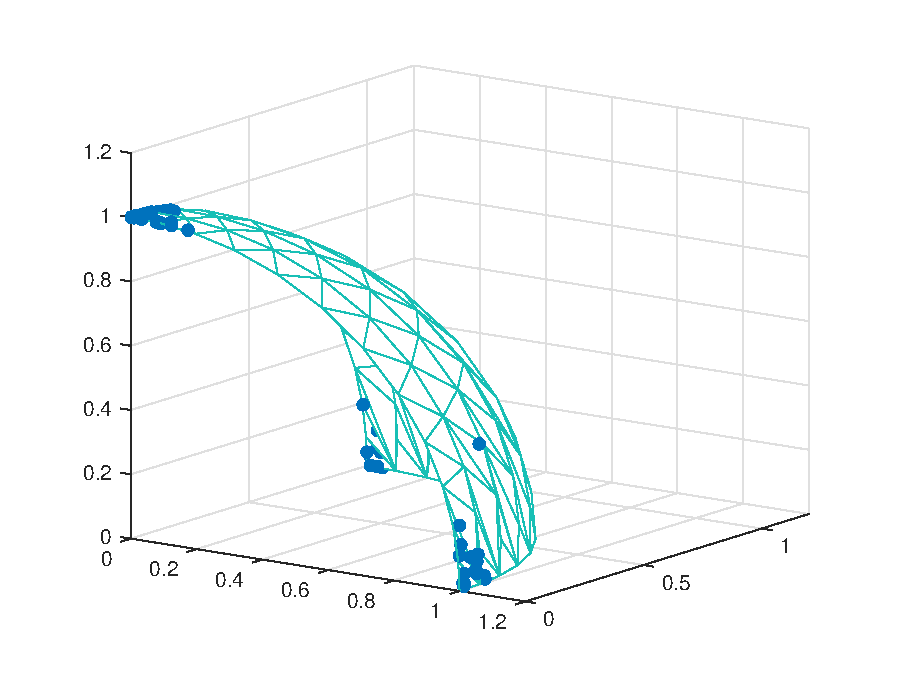
\includegraphics[height=6.45cm]{Figures/nsga_dtlz2_side.eps}\llap{\raisebox{3.1cm}{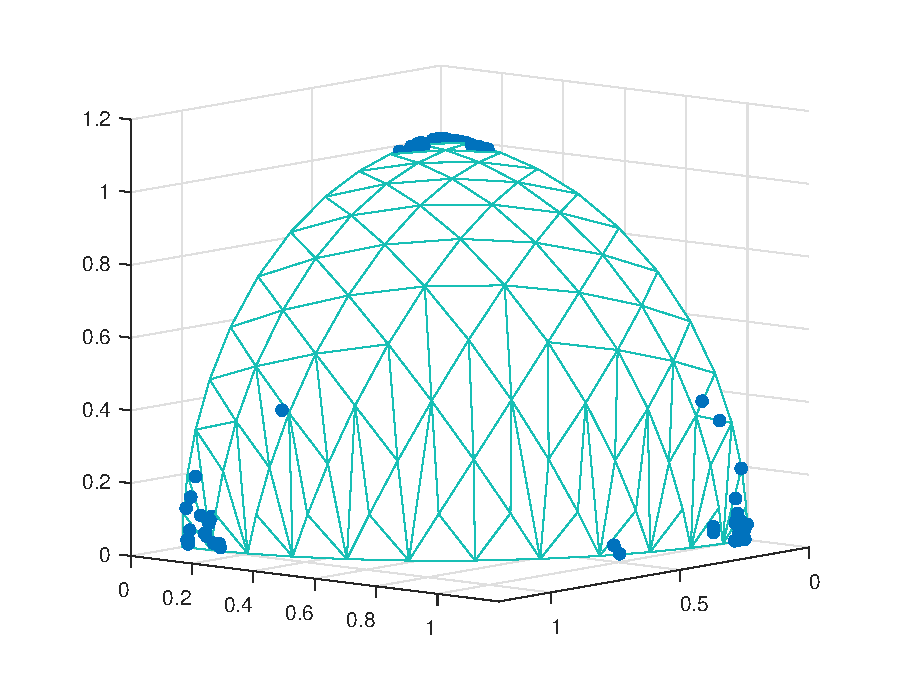
\includegraphics[height=3.1cm]{Figures/nsga_dtlz2.eps}}}
\caption{Najbolja rješenja pronađena pomoću NSGA na DTLZ2}
\label{fig:nsga_dtlz2}
\end{figure}

\begin{figure}[htb]
\centering
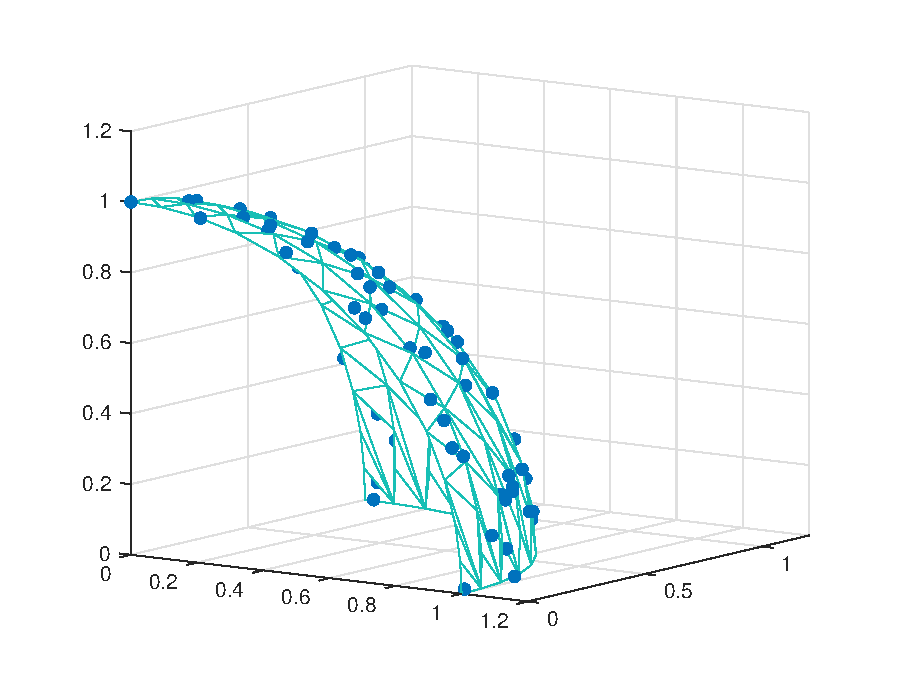
\includegraphics[height=6.45cm]{Figures/nsga2_dtlz2_side.eps}\llap{\raisebox{3.1cm}{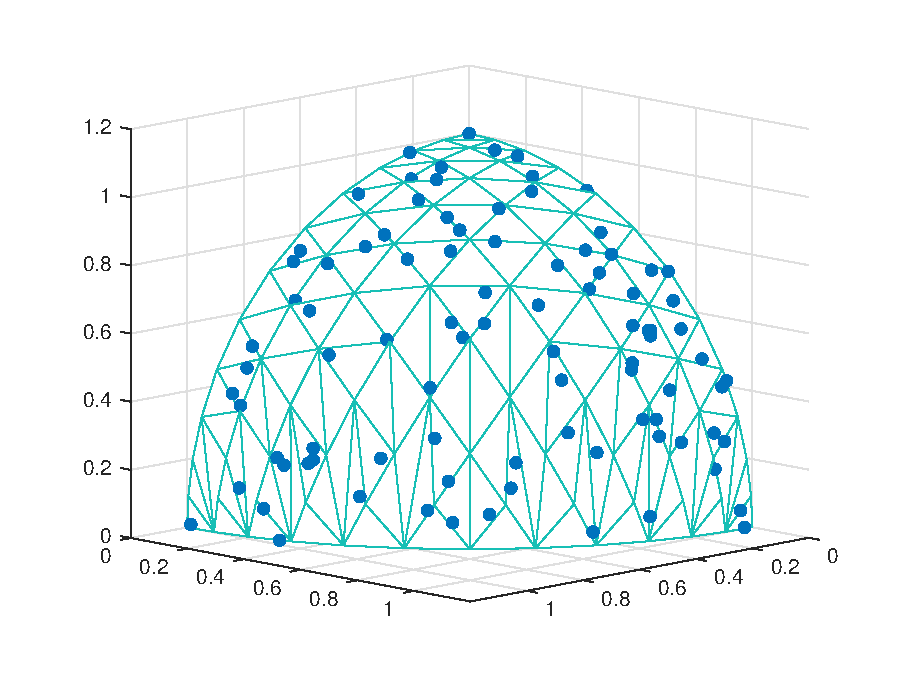
\includegraphics[height=3.1cm]{Figures/nsga2_dtlz2.eps}}}
\caption{Najbolja rješenja pronađena pomoću NSGA-II na DTLZ2}
\label{fig:nsgaii_dtlz2}
\end{figure}

\begin{figure}[htb]
\centering
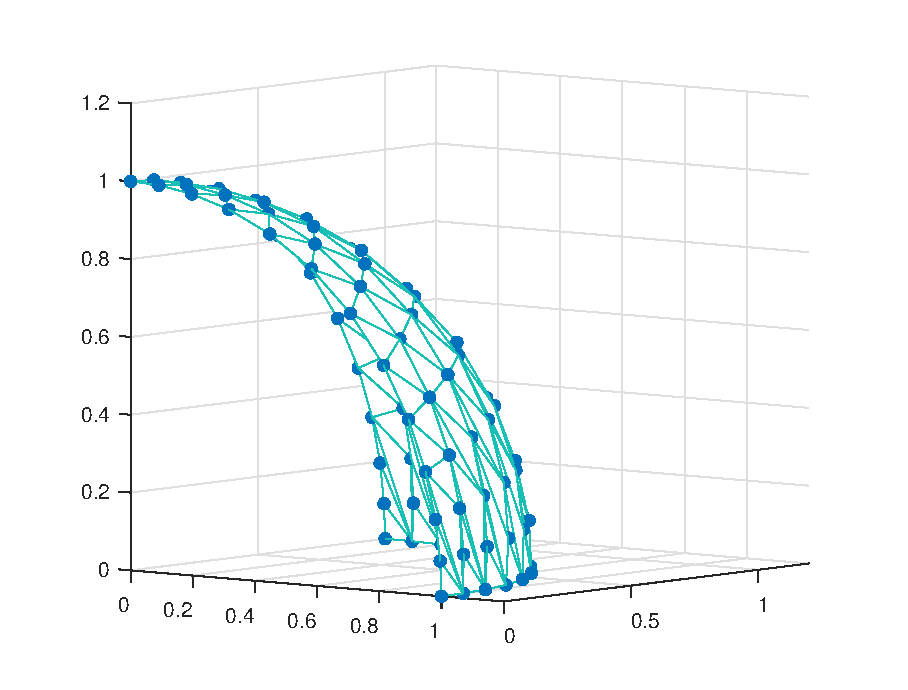
\includegraphics[height=6.45cm]{Figures/nsga3_dtlz2_side.eps}\llap{\raisebox{3.1cm}{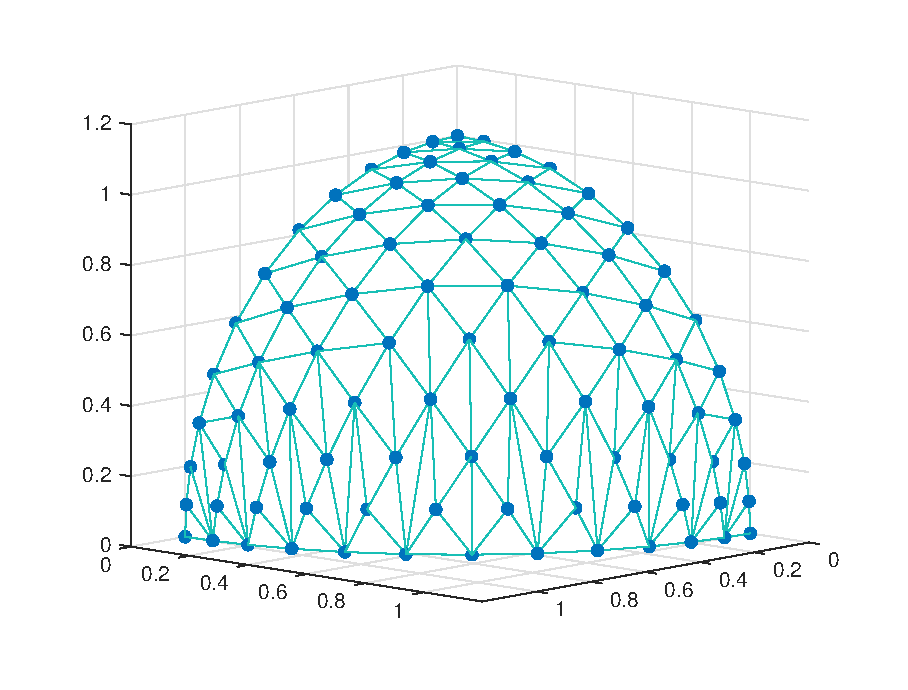
\includegraphics[height=3.1cm]{Figures/nsga3_dtlz2.eps}}}
\caption{Najbolja rješenja pronađena pomoću NSGA-III na DTLZ2}
\label{fig:nsgaiii_dtlz2}
\end{figure}

\begin{figure}[htb]
\centering
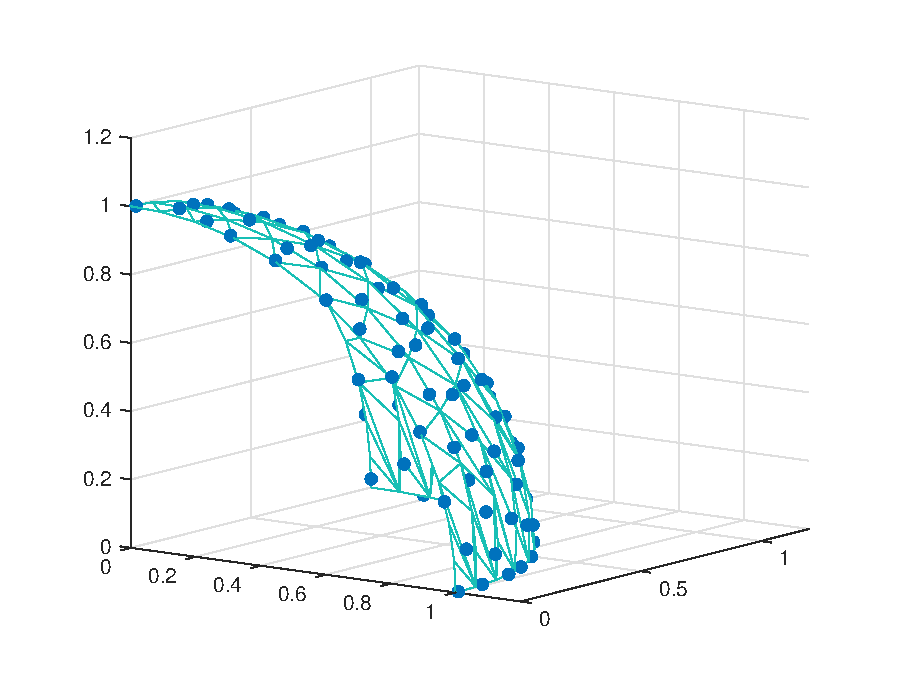
\includegraphics[height=6.45cm]{Figures/spea2_dtlz2_side.eps}\llap{\raisebox{3.1cm}{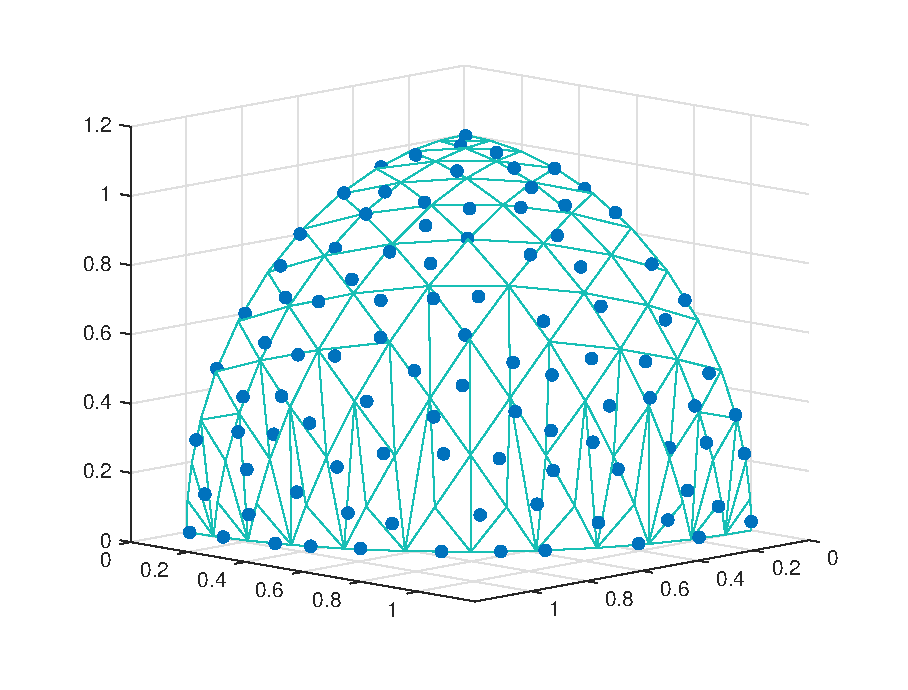
\includegraphics[height=3.1cm]{Figures/spea2_dtlz2.eps}}}
\caption{Najbolja rješenja pronađena pomoću SPEA2 na DTLZ2}
\label{fig:spea2_dtlz2}
\end{figure}

\begin{figure}[htb]
\centering
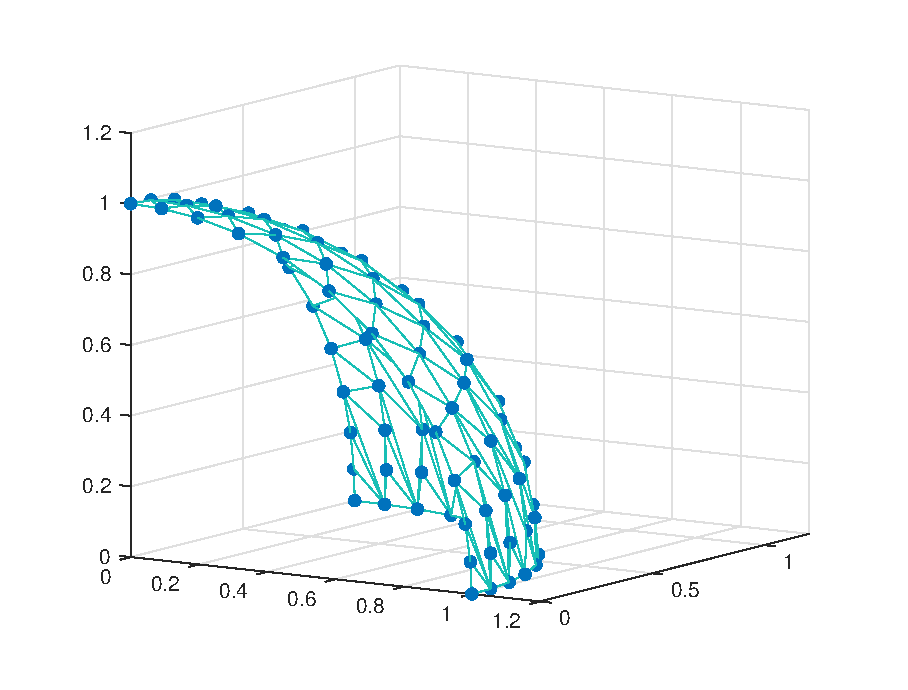
\includegraphics[height=6.45cm]{Figures/moead_pbi_dtlz2_side.eps}\llap{\raisebox{3.1cm}{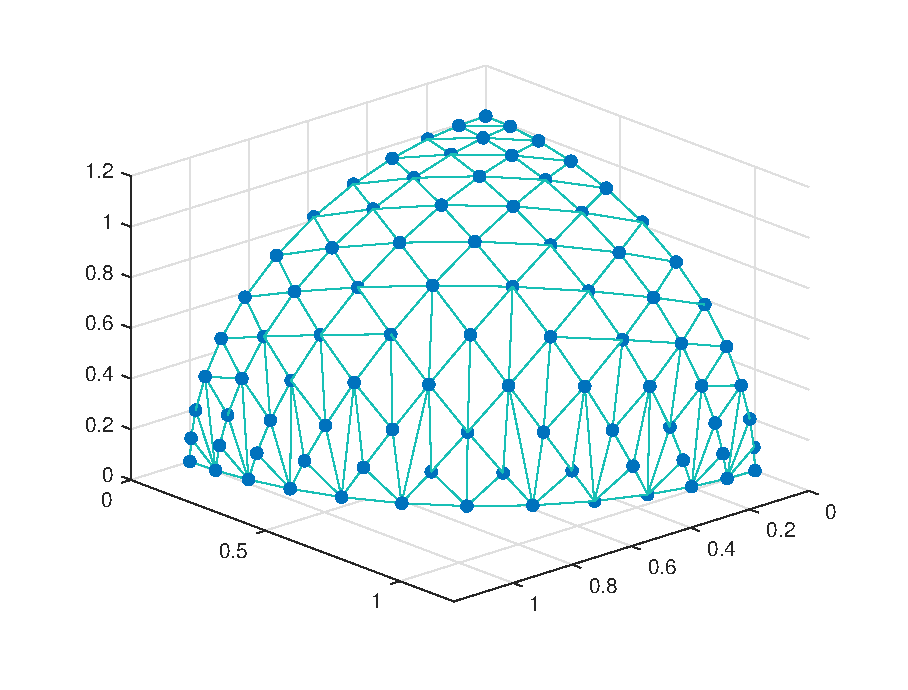
\includegraphics[height=3.1cm]{Figures/moead_pbi_dtlz2.eps}}}
\caption{Najbolja rješenja pronađena pomoću MOEA/D-PBI na DTLZ2}
\label{fig:moeadpbi_dtlz2}
\end{figure}
NSGA se još jednom ispostavlja kao najgori algoritam, pronašavši samo manje grupe točaka lokalizirane na dijelovima Pareto fronte. SPEA2 i NSGA-II pronalaze dobro raspoređene točke, ali ni blizu kao NSGA-III i MOEA/D-PBI koji i na ovom problemu pokazuju najbolju konvergenciju i dobru raznolikost. MOEA/D-TCH, kao i u prethodnom problemu, ima poteškoća s očuvanjem raznovrsnosti rješenja, polučivši lošiji rezultat od NSGA-II i SPEA2. Pregled IGD vrijednosti za sve spomenute algoritme navedene u ovom radu za različite veličine ovog problema nalazi se u tablici \ref{tbl:dtlz2}.
\FloatBarrier	
\begin{figure}[htbp]
\centering
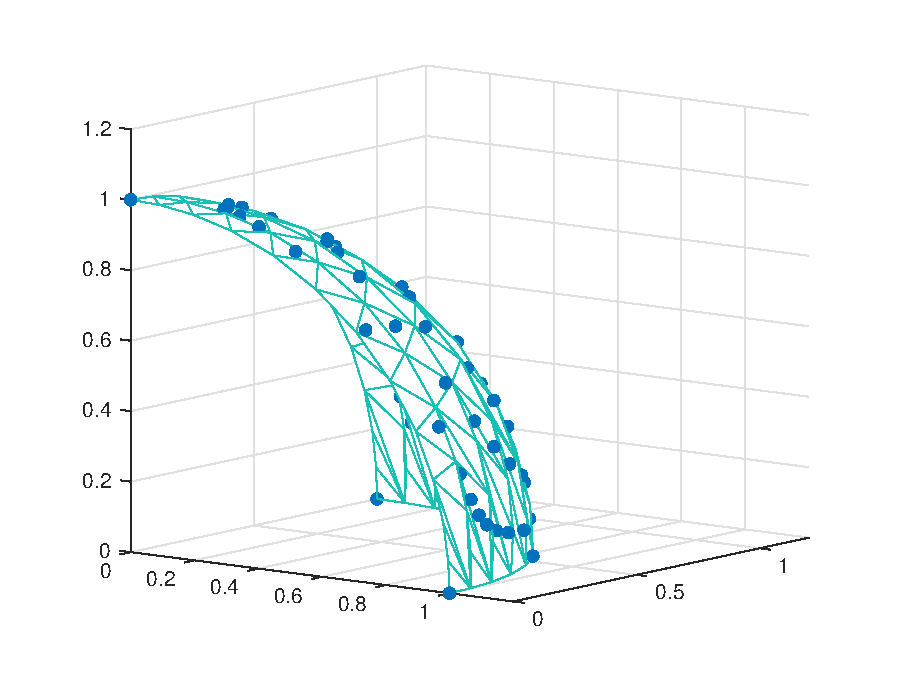
\includegraphics[height=6.45cm]{Figures/moead_tch_dtlz2_side.eps}\llap{\raisebox{3.1cm}{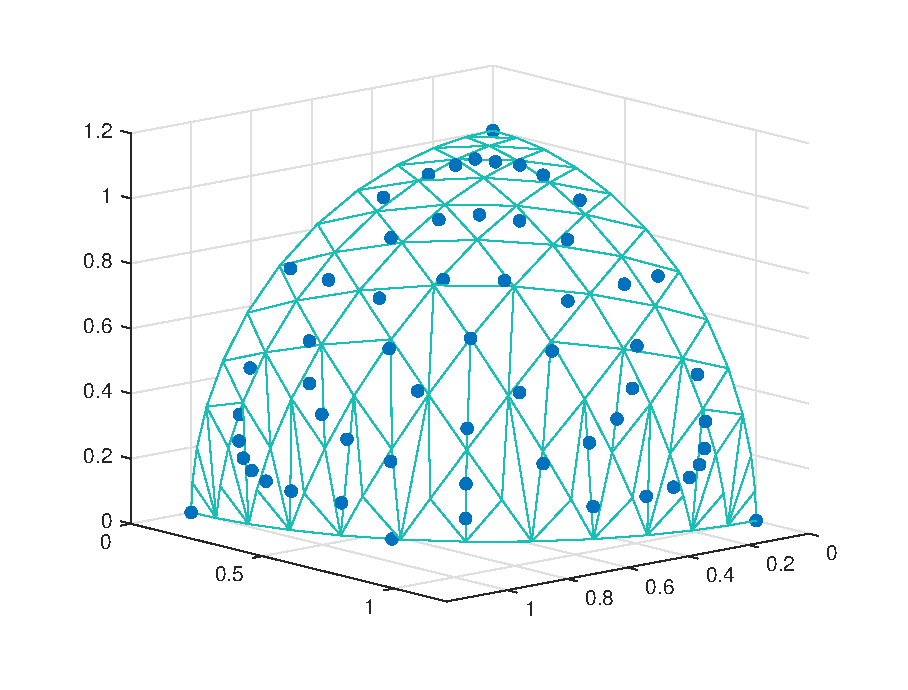
\includegraphics[height=3cm]{Figures/moead_tch_dtlz2.eps}}}
\caption{Najbolja rješenja pronađena pomoću MOEA/D-TCH na DTLZ2}
\label{fig:moeadtch_dtlz2}
\end{figure}
 


\begin{table}[htb]
\caption{IGD vrijednosti algoritama za problem DTLZ2}
\label{tbl:dtlz2}
\centering
\small
\begin{tabular}{c|c|c|c|c|c|c} \hline
$M$ & NSGA & NSGA-II & NSGA-III & SPEA2 & MOEA/D-PBI & MOEA/D-TCH  \\ \hline
\multirow{3}{*}{2}  & $8.467\times 10^{-2}$    & $4.955\times 10^{-3}$ & $4.370\times 10^{-4}$ & $3.592\times 10^{-3}$ & $1.652\times 10^{-4}$ & $\mathbf{1.345\times 10^{-4}}$\\
			        & $1.432\times 10^{-1}$    & $5.558\times 10^{-3}$ & $1.347\times 10^{-3}$ & $4.297\times 10^{-3}$ & $4.957\times 10^{-4}$ & $\mathbf{3.357\times 10^{-4}}$\\
                    & $1.785\times 10^{-1}$    & $6.264\times 10^{-3}$ & $6.768\times 10^{-3}$ & $5.415\times 10^{-3}$ & $1.394\times 10^{-3}$ & $\mathbf{1.219\times 10^{-3}}$\\ \hline
\multirow{3}{*}{3}  & $2.296\times 10^{-1}$    & $6.663\times 10^{-2}$ & $1.750\times 10^{-4}$ & $4.690\times 10^{-2}$ & $\mathbf{1.481\times 10^{-4}}$ & $7.769\times 10^{-2}$\\
			        & $2.551\times 10^{-1}$    & $7.432\times 10^{-2}$ & $2.221\times 10^{-4}$ & $5.354\times 10^{-2}$ & $\mathbf{1.913\times 10^{-4}}$ & $7.990\times 10^{-2}$\\
                    & $3.074\times 10^{-1}$    & $8.210\times 10^{-2}$ & $\mathbf{2.732\times 10^{-4}}$ & $7.650\times 10^{-2}$ & $3.325\times 10^{-4}$ & $8.046\times 10^{-2}$\\ \hline
\multirow{3}{*}{5}  & $3.607\times 10^{-1}$    & $1.948\times 10^{-1}$ & $\mathbf{4.132\times 10^{-4}}$ & $2.023\times 10^{-1}$ & $9.664\times 10^{-3}$ & $4.091\times 10^{-1}$\\
			        & $3.861\times 10^{-1}$    & $2.024\times 10^{-1}$ & $\mathbf{4.577\times 10^{-4}}$ & $2.082\times 10^{-1}$ & $1.164\times 10^{-2}$ & $4.379\times 10^{-1}$\\
                    & $4.258\times 10^{-1}$    & $2.113\times 10^{-1}$ & $\mathbf{5.326\times 10^{-4}}$ & $2.421\times 10^{-1}$ & $1.588\times 10^{-2}$ & $4.622\times 10^{-1}$\\ \hline
\multirow{3}{*}{8}  & $5.243\times 10^{-1}$    & $3.604\times 10^{-1}$ & $\mathbf{1.904\times 10^{-3}}$ & $3.811\times 10^{-1}$ & $3.121\times 10^{-2}$ & $5.891\times 10^{-1}$\\
			        & $5.803\times 10^{-1}$    & $3.701\times 10^{-1}$ & $\mathbf{2.185\times 10^{-3}}$ & $3.919\times 10^{-1}$ & $3.926\times 10^{-2}$ & $6.570\times 10^{-1}$\\
                    & $6.424\times 10^{-1}$    & $3.799\times 10^{-1}$ & $\mathbf{3.675\times 10^{-3}}$ & $4.305\times 10^{-1}$ & $4.560\times 10^{-2}$ & $6.904\times 10^{-1}$\\ \hline
\multirow{3}{*}{10} & $5.751\times 10^{-1}$    & $4.013\times 10^{-1}$ & $\mathbf{2.837\times 10^{-3}}$ & $4.662\times 10^{-1}$ & $6.934\times 10^{-2}$ & $7.301\times 10^{-1}$\\
			        & $6.408\times 10^{-1}$    & $4.098\times 10^{-1}$ & $\mathbf{3.219\times 10^{-3}}$ & $5.026\times 10^{-1}$ & $7.768\times 10^{-2}$ & $7.577\times 10^{-1}$\\
                    & $6.848\times 10^{-1}$    & $4.190\times 10^{-1}$ & $\mathbf{3.548\times 10^{-3}}$ & $5.839\times 10^{-1}$ & $8.568\times 10^{-2}$ & $7.895\times 10^{-1}$\\ \hline
\end{tabular}
\end{table}
Iz tablice možemo primijetiti da se rezultati razlikuju u određenoj mjeri od onih za DTLZ1 --- povećavanjem broja ciljnih funkcija, NSGA-III daje značajno bolje rezultate nego ostali algoritmi. Oba pristupa MOEA/D pronalaze dobar skup rješenja samo za manje probleme, dok za veće, to nisu u mogućnosti. Treba također primijetiti da, osim NSGA-III i MOEA/D-PBI, za veće dimenzije problema algoritmi pronalaze loše skupove rješenja, tj. loše aproksimiraju Pareto frontu.

\FloatBarrier
\subsection{DTLZ3} 
Višekriterijski problem DTLZ3 definiran je na sljedeći način:
\begin{align*}
\mbox{Minimiziraj }\: &f_1(\vec{x}) = (1 + g(\vec{x}_M))\cos{(x_1\pi/2)}\cos{(x_2\pi/2)}\cdots\cos{(x_{M - 2}\pi/2)}\cos{(x_{M - 1}\pi/2)},\\
\mbox{Minimiziraj }\: &f_2(\vec{x}) = (1 + g(\vec{x}_M))\cos{(x_1\pi/2)}\cos{(x_2\pi/2)}\cdots\cos{(x_{M - 2}\pi/2)}\sin{(x_{M - 1}\pi/2)},\\
\mbox{Minimiziraj }\: &f_3(\vec{x}) = (1 + g(\vec{x}_M))\cos{(x_1\pi/2)}\cos{(x_2\pi/2)}\cdots\sin{(x_{M - 2}\pi/2)},\\
\vdots\\
\mbox{Minimiziraj }\: &f_{M-1}(\vec{x}) = (1 + g(\vec{x}_M))\cos{(x_1\pi/2)}\sin{(x_2\pi/2)},\\
\mbox{Minimiziraj }\: &f_{M}(\vec{x}) = (1 + g(\vec{x}_M))\sin{(x_1\pi/2)},\\
\mbox{uz ograničenja }\: &0 \leq x_i \leq 1, \quad \text{za } i = 1,\dots, n,\\
\mbox{gdje je }\: &g(\vec{x}_M) = \sum_{x_i \in \vec{x}_M}{(x_i - 0.5)^2}.
\end{align*}
Primijetimo da je jedina razlika između DTLZ3 i DTLZ2 u funkciji $g(\vec{x}_M)$ --- u DTLZ3 koristimo izraz \ref{eq:cos_g}. Autori predlažu $k = \vert\vec{x}_M\vert = 10$. Funkcijom \ref{eq:cos_g} uvodimo $3^k - 1$ lokalnih Pareto fronti te jednu globalnu koja je jednaka onoj u DTLZ2. Ovaj problem ispituje sposobnost algoritma da konvergira globalnoj Pareto fronti. Rezultati algoritama za DTLZ3 s 3 ciljne funkcije prikazane su na slikama \ref{fig:nsga_dtlz3} -- \ref{fig:moeadtch_dtlz3}.\\

\begin{figure}[htb]
\centering
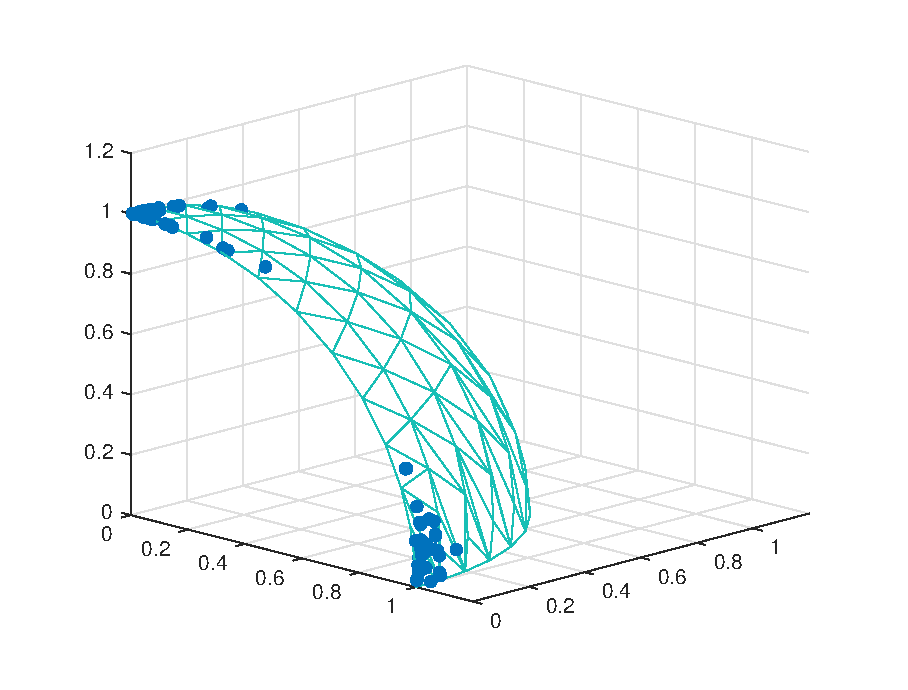
\includegraphics[height=6.45cm]{Figures/nsga_dtlz3_side.eps}\llap{\raisebox{3.1cm}{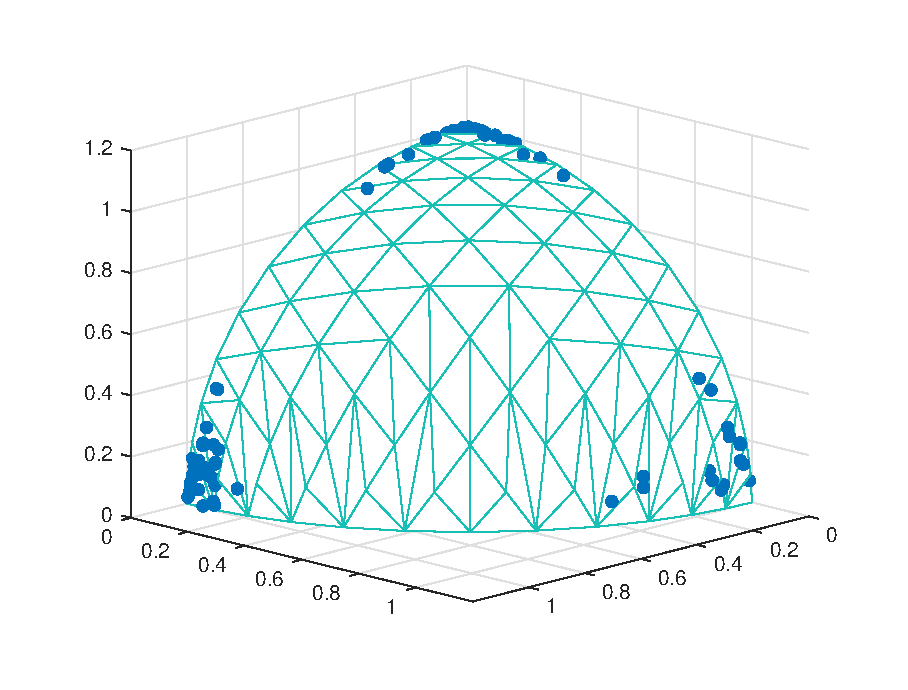
\includegraphics[height=3.1cm]{Figures/nsga_dtlz3.eps}}}
\caption{Najbolja rješenja pronađena pomoću NSGA na DTLZ3}
\label{fig:nsga_dtlz3}
\end{figure}

\begin{figure}[htb]
\centering
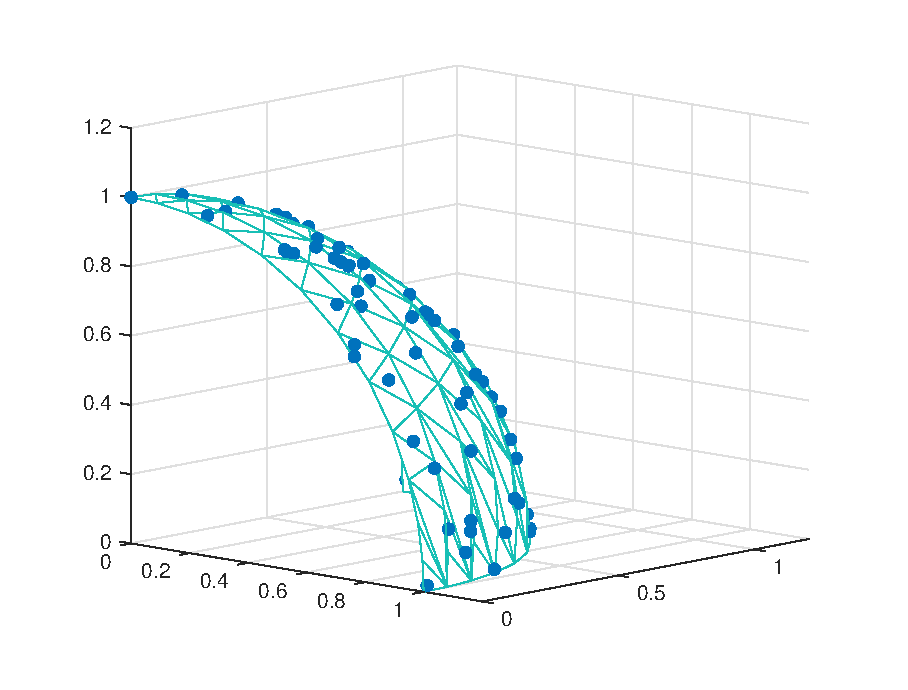
\includegraphics[height=6.45cm]{Figures/nsga2_dtlz3_side.eps}\llap{\raisebox{3.1cm}{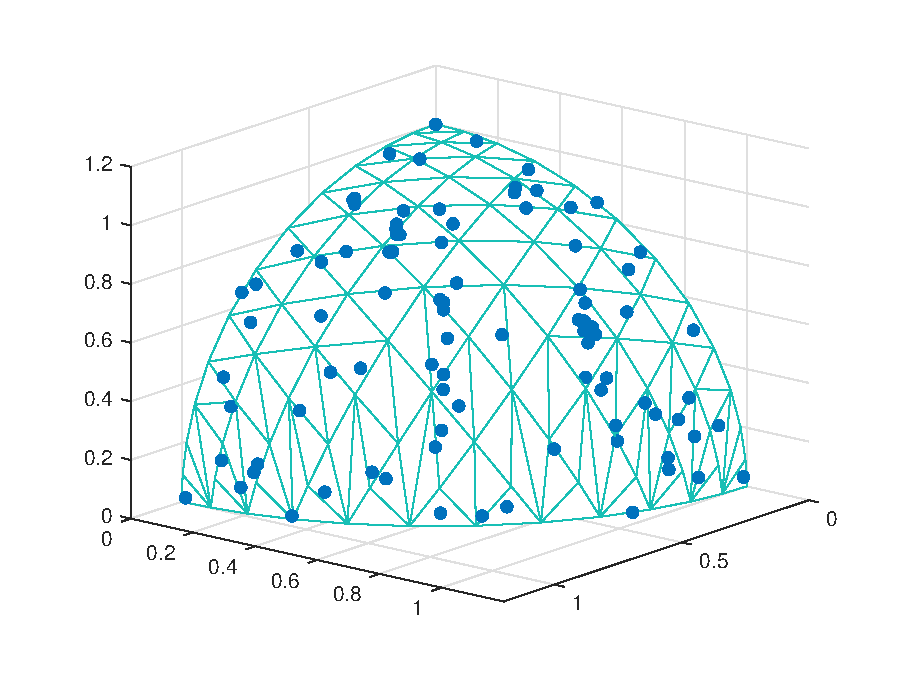
\includegraphics[height=3.1cm]{Figures/nsga2_dtlz3.eps}}}
\caption{Najbolja rješenja pronađena pomoću NSGA-II na DTLZ3}
\label{fig:nsgaii_dtlz3}
\end{figure}

\begin{figure}[htb]
\centering
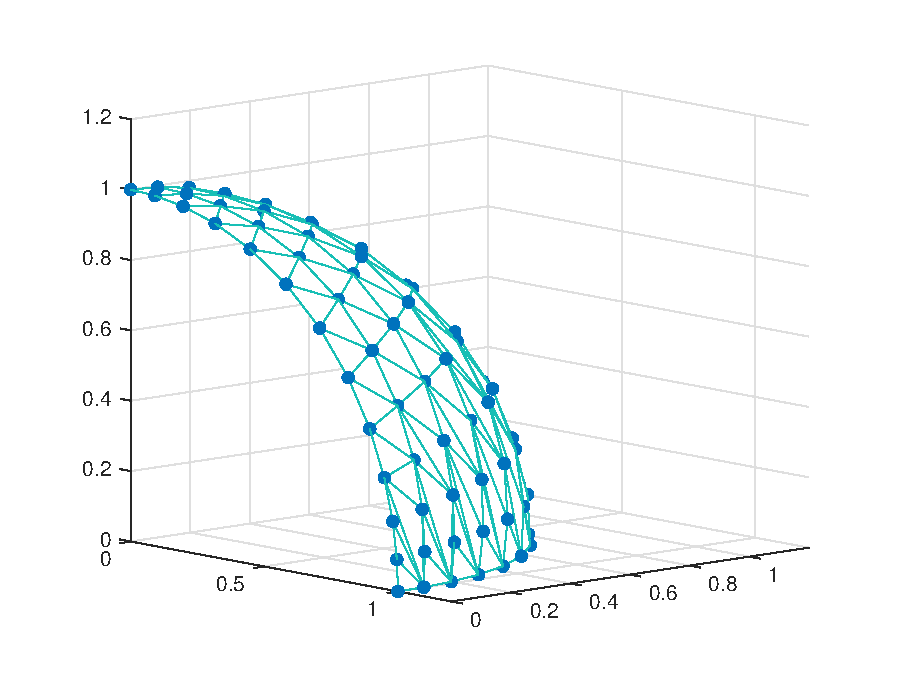
\includegraphics[height=6.45cm]{Figures/nsga3_dtlz3_side.eps}\llap{\raisebox{3.1cm}{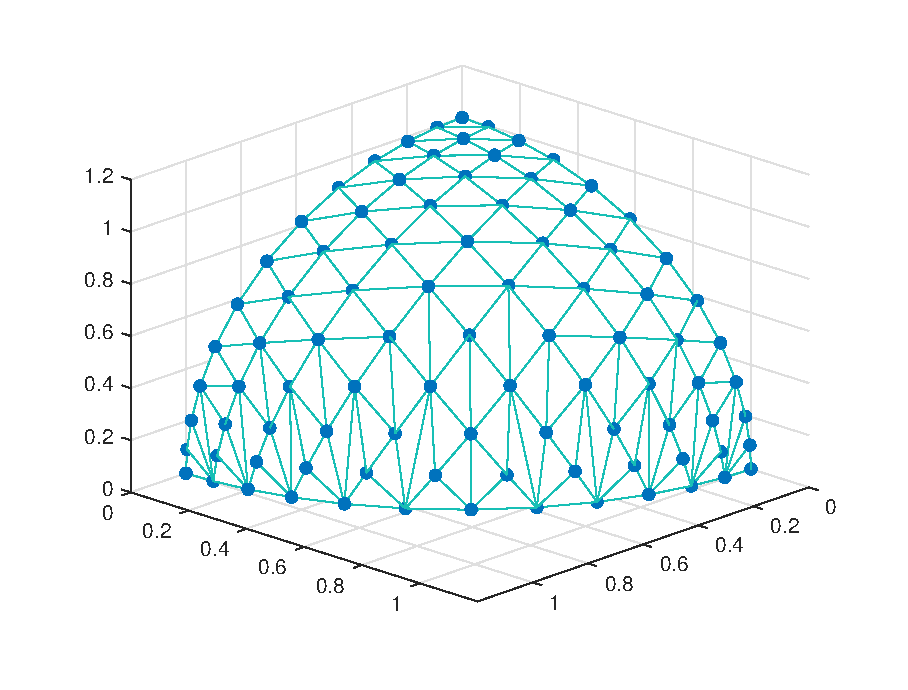
\includegraphics[height=3.1cm]{Figures/nsga3_dtlz3.eps}}}
\caption{Najbolja rješenja pronađena pomoću NSGA-III na DTLZ3}
\label{fig:nsgaiii_dtlz3}
\end{figure}

\begin{figure}[htb]
\centering
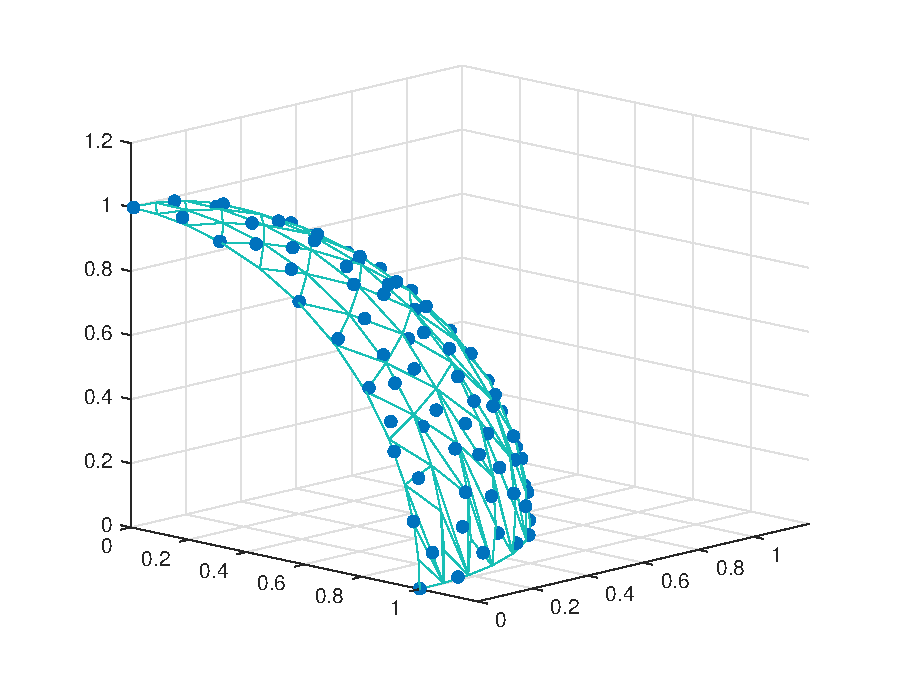
\includegraphics[height=6.45cm]{Figures/spea2_dtlz3_side.eps}\llap{\raisebox{3.1cm}{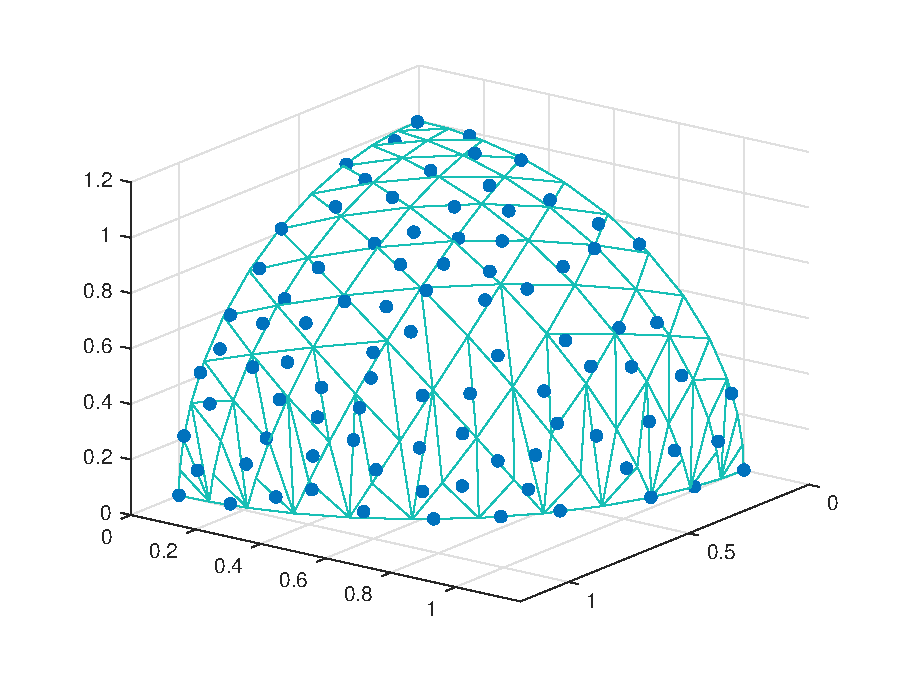
\includegraphics[height=3.1cm]{Figures/spea2_dtlz3.eps}}}
\caption{Najbolja rješenja pronađena pomoću SPEA2 na DTLZ3}
\label{fig:spea2_dtlz3}
\end{figure}

\begin{figure}[htb]
\centering
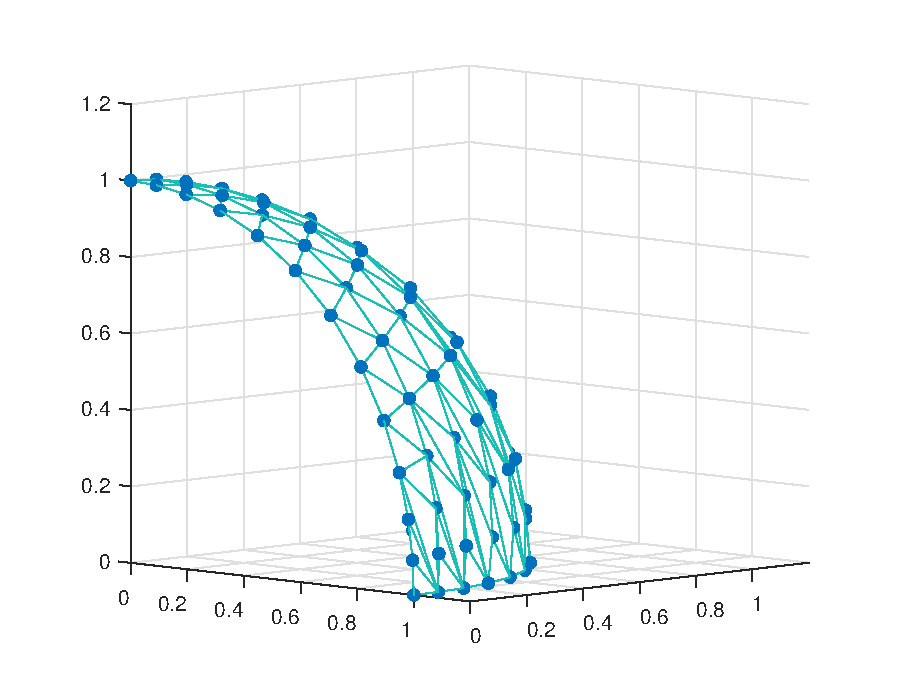
\includegraphics[height=6.45cm]{Figures/moead_pbi_dtlz3_side.eps}\llap{\raisebox{3.1cm}{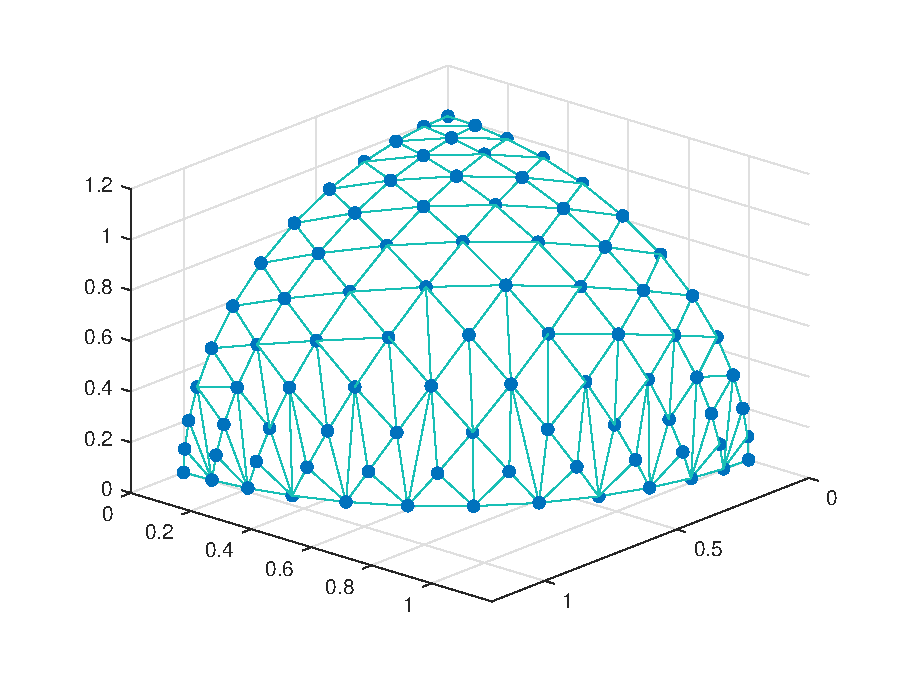
\includegraphics[height=3.1cm]{Figures/moead_pbi_dtlz3.eps}}}
\caption{Najbolja rješenja pronađena pomoću MOEA/D-PBI na DTLZ3}
\label{fig:moeadpbi_dtlz3}
\end{figure}

Iako se ispostavlja da NSGA može konvergirati globalnoj Pareto fronti, ne pokazuje se nikakav napredak u raznolikosti odnosu na prethodne probleme --- još uvijek se pronađena rješenja nalaze u grupicama na izoliranim dijelovima Pareto fronte. S druge strane, NSGA-II, SPEA2 i MOEA/D-TCH pokazuju bolju raznovrsnost točaka, gdje, od navedenih algoritama, SPEA2 pokazuje najbolju. Međutim, NSGA-III i MOEA/D-PBI pokazuju se još jednom kao apsolutni pobjednici gotovo optimalnom konvergencijom i raznolikošću rješenja. \\
U tablici \ref{tbl:dtlz3} nalaze se IGD vrijednosti algoritama za DTLZ3 različite veličine.
\FloatBarrier
\begin{figure}[htb]
\centering
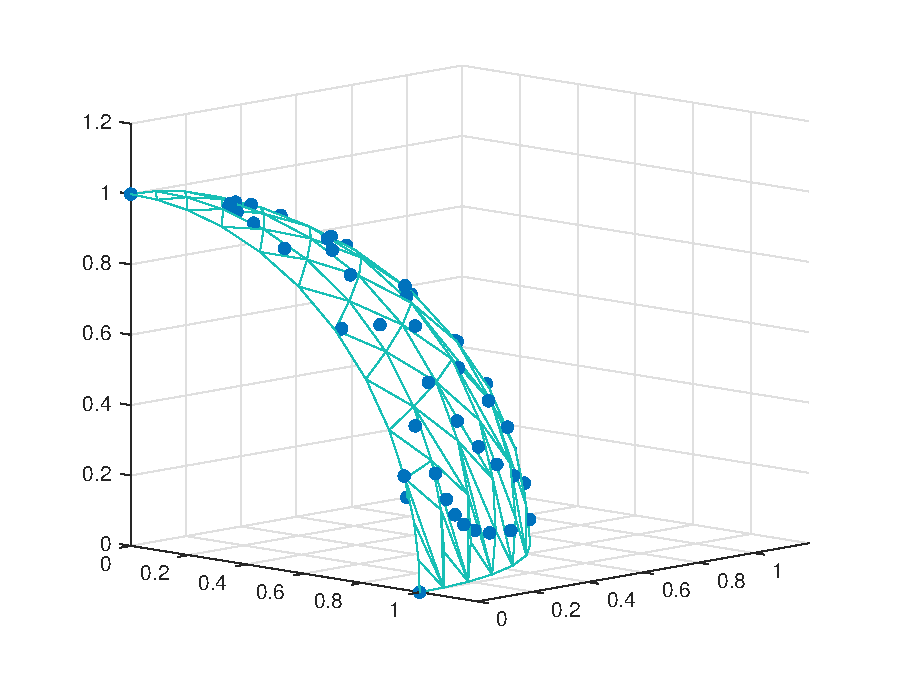
\includegraphics[height=6.45cm]{Figures/moead_tch_dtlz3_side.eps}\llap{\raisebox{3.1cm}{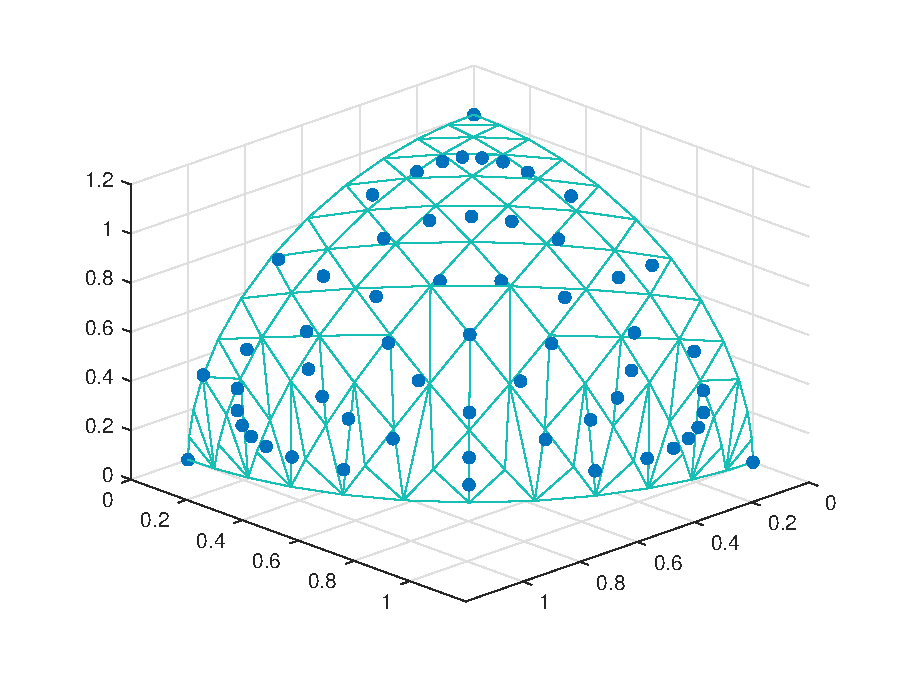
\includegraphics[height=3.1cm]{Figures/moead_tch_dtlz3.eps}}}
\caption{Najbolja rješenja pronađena pomoću MOEA/D-TCH na DTLZ3}
\label{fig:moeadtch_dtlz3}
\end{figure} 

\begin{table}[htb]
\caption{IGD vrijednosti algoritama za problem DTLZ3}
\label{tbl:dtlz3}
\centering
\small
\begin{tabular}{c|c|c|c|c|c|c} \hline
$M$ & NSGA & NSGA-II & NSGA-III & SPEA2 & MOEA/D-PBI & MOEA/D-TCH  \\ \hline
\multirow{3}{*}{2}  & $5.915\times 10^{-2}$    & $4.662\times 10^{-3}$ & $3.895\times 10^{-4}$ & $3.454\times 10^{-3}$ & $\mathbf{1.256\times 10^{-4}}$ &  $1.394\times 10^{-4}$\\
			        & $1.277\times 10^{-1}$    & $5.369\times 10^{-3}$ & $1.251\times 10^{-3}$ & $4.300\times 10^{-3}$ & $5.154\times 10^{-4}$ & $\mathbf{3.823\times 10^{-4}}$\\
                    & $2.001\times 10^{-1}$    & $6.106\times 10^{-3}$ & $4.315\times 10^{-3}$ & $5.892\times 10^{-3}$ & $1.549\times 10^{-3}$ & $\mathbf{1.500\times 10^{-3}}$\\ \hline
\multirow{3}{*}{3}  & $1.957\times 10^{-1}$    & $7.026\times 10^{-2}$ & $1.852\times 10^{-4}$ & $5.223\times 10^{-2}$ & $\mathbf{1.398\times 10^{-4}}$ & $7.804\times 10^{-2}$\\
			        & $2.470\times 10^{-1}$    & $7.410\times 10^{-2}$ & $2.338\times 10^{-4}$ & $5.768\times 10^{-2}$ & $\mathbf{1.871\times 10^{-4}}$ & $7.952\times 10^{-2}$\\
                    & $3.005\times 10^{-1}$    & $8.202\times 10^{-2}$ & $3.874\times 10^{-4}$ & $7.178\times 10^{-2}$ & $\mathbf{2.760\times 10^{-4}}$ & $8.045\times 10^{-2}$\\ \hline
\multirow{3}{*}{5}  & $3.518\times 10^{-1}$    & $1.954\times 10^{-1}$ & $\mathbf{4.134\times 10^{-4}}$ & $2.018\times 10^{-1}$ & $8.654\times 10^{-3}$ & $4.077\times 10^{-1}$\\
			        & $3.803\times 10^{-1}$    & $2.039\times 10^{-1}$ & $\mathbf{4.563\times 10^{-4}}$ & $2.129\times 10^{-1}$ & $1.195\times 10^{-2}$ & $4.353\times 10^{-1}$\\
                    & $3.958\times 10^{-1}$    & $2.178\times 10^{-1}$ & $\mathbf{5.534\times 10^{-4}}$ & $2.390\times 10^{-1}$ & $1.516\times 10^{-2}$ & $4.577\times 10^{-1}$\\ \hline
\multirow{3}{*}{8}  & $5.310\times 10^{-1}$    & $3.582\times 10^{-1}$ & $\mathbf{2.046\times 10^{-3}}$ & $3.720\times 10^{-1}$ & $3.071\times 10^{-2}$ & $5.996\times 10^{-1}$\\
			        & $5.606\times 10^{-1}$    & $3.708\times 10^{-1}$ & $\mathbf{2.377\times 10^{-3}}$ & $3.979\times 10^{-1}$ & $3.938\times 10^{-2}$ & $6.522\times 10^{-1}$\\
                    & $6.232\times 10^{-1}$    & $3.810\times 10^{-1}$ & $\mathbf{2.742\times 10^{-3}}$ & $4.309\times 10^{-1}$ & $4.677\times 10^{-2}$ & $6.766\times 10^{-1}$\\ \hline
\multirow{3}{*}{10} & $5.926\times 10^{-1}$    & $4.042\times 10^{-1}$ & $\mathbf{2.824\times 10^{-3}}$ & $4.586\times 10^{-1}$ & $7.012\times 10^{-2}$ & $7.256\times 10^{-1}$\\
			        & $6.501\times 10^{-1}$    & $4.116\times 10^{-1}$ & $\mathbf{3.144\times 10^{-3}}$ & $4.985\times 10^{-1}$ & $7.608\times 10^{-2}$ & $7.497\times 10^{-1}$\\
                    & $7.112\times 10^{-1}$    & $4.235\times 10^{-1}$ & $\mathbf{3.910\times 10^{-3}}$ & $5.627\times 10^{-1}$ & $8.250\times 10^{-2}$ & $7.875\times 10^{-1}$\\ \hline
\end{tabular}
\end{table}
Kako vidimo iz tablice, za veći broj ciljnih funkcija MOEA/D-TCH, NSGA, NSGA-II i SPEA2 daju slične IGD vrijednosti koje su vrlo loše te će se izostaviti iz daljnjeg razmatranja kod DTLZ3. NSGA-III, s druge strane, ostvaruje vrlo dobre rezultate za DTLZ3 većih dimenzija što ide u prilog njegovoj sposobnosti konvergencije globalnoj Pareto fronti. MOEA/D-PBI također daje prihvatljive rezultate, ali znatno lošije od onih koje pronalazi NSGA-III.

\FloatBarrier
\subsection{DTLZ4}
Višekriterijski problem DTLZ4 definiran je na sljedeći način:
\begin{align*}
\mbox{Minimiziraj }\: &f_1(\vec{x}) = (1 + g(\vec{x}_M))\cos{(x_1^{\alpha}\pi/2)}\cos{(x_2^{\alpha}\pi/2)}\cdots\cos{(x_{M - 2}^{\alpha}\pi/2)}\cos{(x_{M - 1}^{\alpha}\pi/2)},\\
\mbox{Minimiziraj }\: &f_2(\vec{x}) = (1 + g(\vec{x}_M))\cos{(x_1^{\alpha}\pi/2)}\cos{(x_2^{\alpha}\pi/2)}\cdots\cos{(x_{M - 2}^{\alpha}\pi/2)}\sin{(x_{M - 1}^{\alpha}\pi/2)},\\
\mbox{Minimiziraj }\: &f_3(\vec{x}) = (1 + g(\vec{x}_M))\cos{(x_1^{\alpha}\pi/2)}\cos{(x_2^{\alpha}\pi/2)}\cdots\sin{(x_{M - 2}^{\alpha}\pi/2)},\\
\vdots\\
\mbox{Minimiziraj }\: &f_{M-1}(\vec{x}) = (1 + g(\vec{x}_M))\cos{(x_1^{\alpha}\pi/2)}\sin{(x_2^{\alpha}\pi/2)},\\
\mbox{Minimiziraj }\: &f_{M}(\vec{x}) = (1 + g(\vec{x}_M))\sin{(x_1^{\alpha}\pi/2)},\\
\mbox{uz ograničenja }\: &0 \leq x_i \leq 1, \quad \text{za } i = 1,\dots, n,\\
\mbox{gdje je }\: &g(\vec{x}_M) = \sum_{x_i \in \vec{x}_M}{(x_i - 0.5)^2}.
\end{align*}
Autori predlažu $\alpha = 100$ te $k = 10$. Ovaj problem je, kao i DTLZ3, sličan DTLZ2, ali postoji jedna bitna razlika: zbog parametra $\alpha$, postoji skup rješenja gusto zbijen uz ravninu $f_M-f_1$ što algoritmu može otežati očuvanje dobre raznolikosti rješenja. Rezultati za DTLZ4 s 3 ciljne funkcije su na slikama \ref{fig:nsga_dtlz4} -- \ref{fig:moeadtch_dtlz4}.\\

\begin{figure}[htb]
\centering
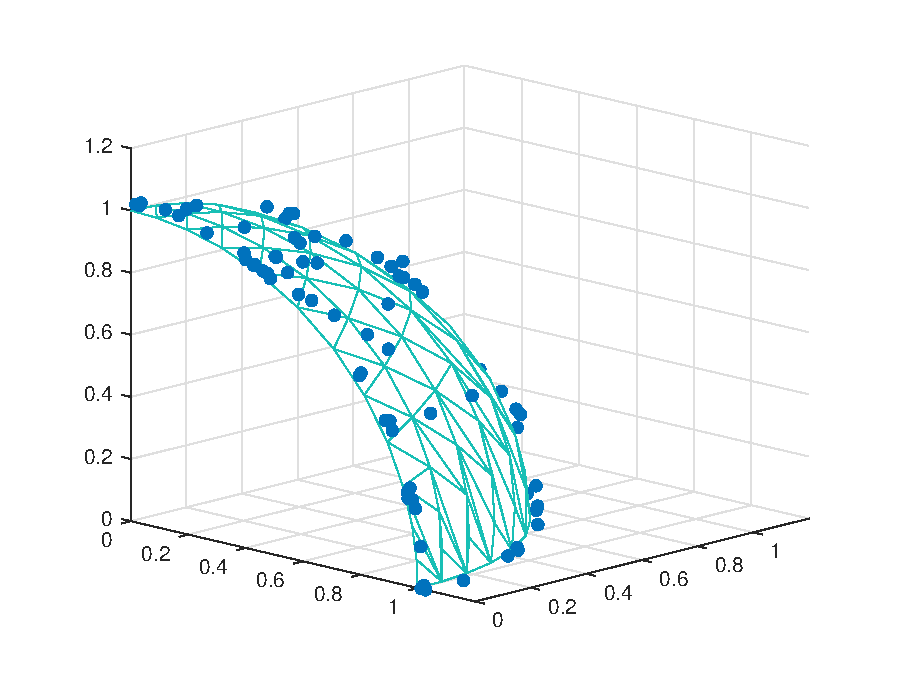
\includegraphics[height=6.45cm]{Figures/nsga_dtlz4_side.eps}\llap{\raisebox{3.1cm}{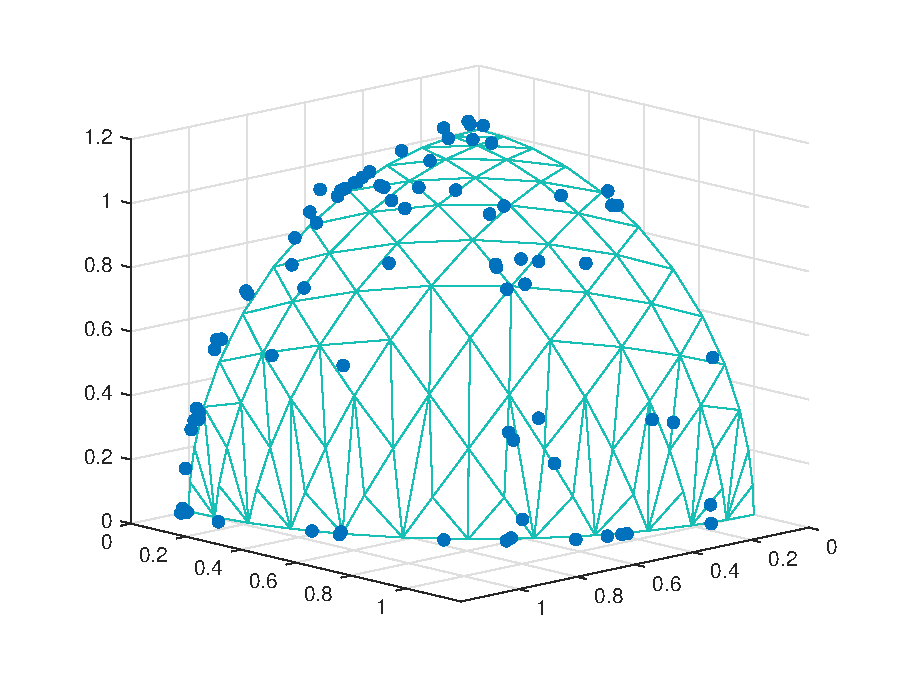
\includegraphics[height=3.1cm]{Figures/nsga_dtlz4.eps}}}
\caption{Najbolja rješenja pronađena pomoću NSGA na DTLZ4}
\label{fig:nsga_dtlz4}
\end{figure}

\begin{figure}[htb]
\centering
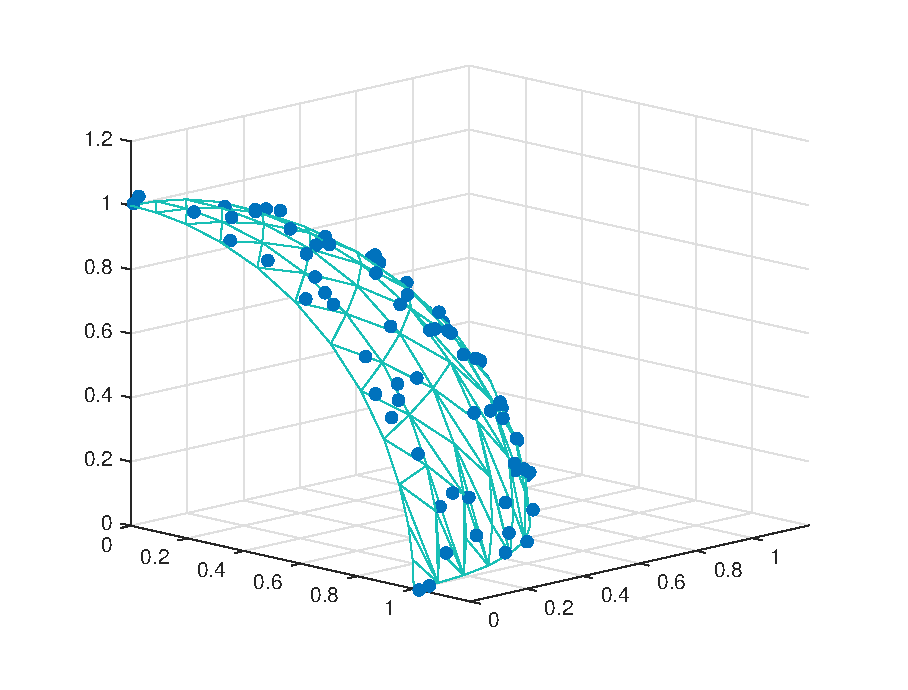
\includegraphics[height=6.45cm]{Figures/nsga2_dtlz4_side.eps}\llap{\raisebox{3.1cm}{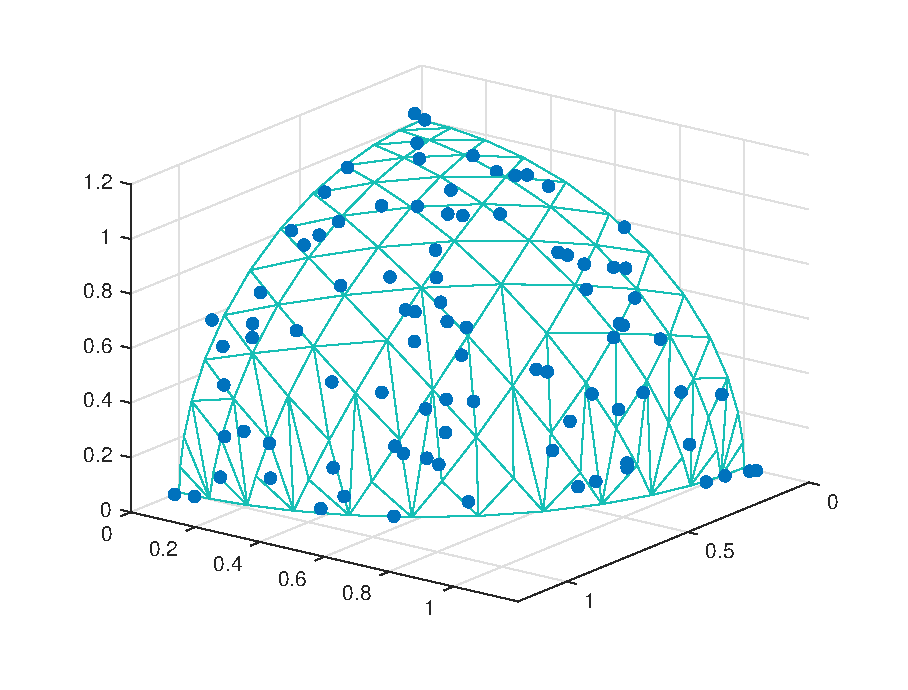
\includegraphics[height=3.1cm]{Figures/nsga2_dtlz4.eps}}}
\caption{Najbolja rješenja pronađena pomoću NSGA-II na DTLZ4}
\label{fig:nsgaii_dtlz4}
\end{figure}

\begin{figure}[htb]
\centering
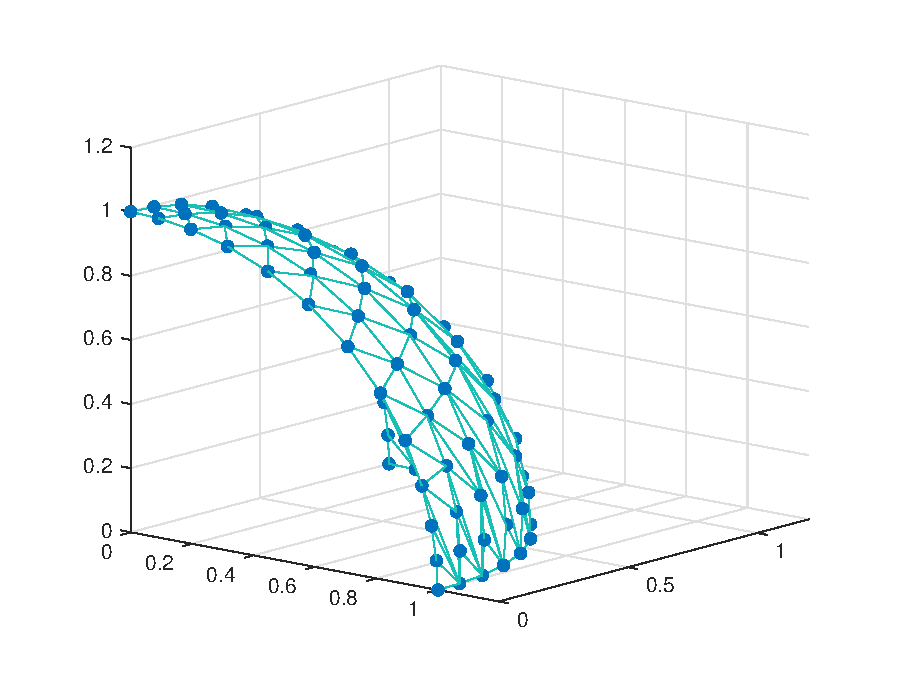
\includegraphics[height=6.45cm]{Figures/nsga3_dtlz4_side.eps}\llap{\raisebox{3.1cm}{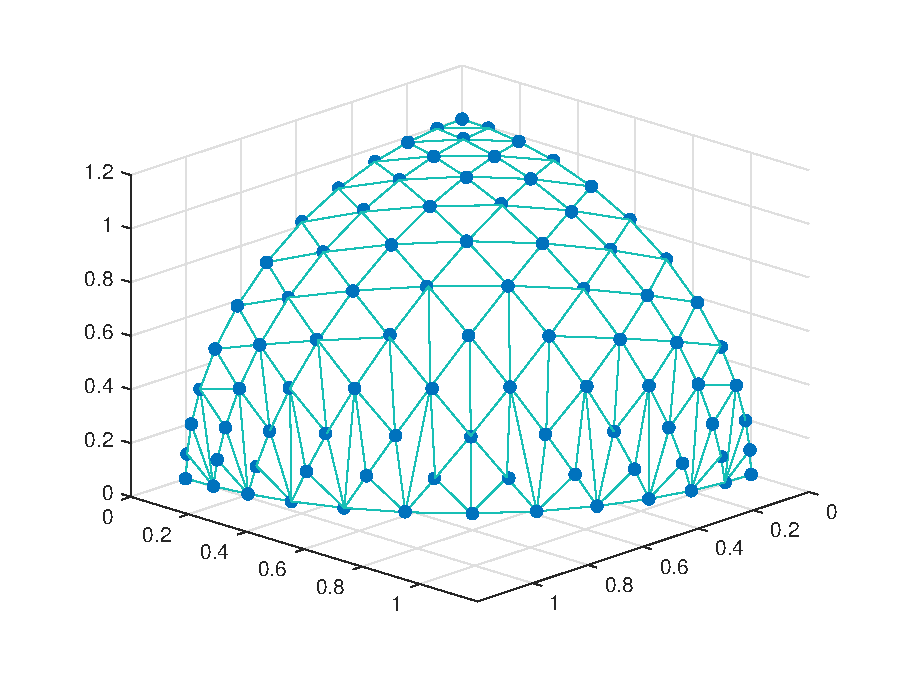
\includegraphics[height=3.1cm]{Figures/nsga3_dtlz4.eps}}}
\caption{Najbolja rješenja pronađena pomoću NSGA-III na DTLZ4}
\label{fig:nsgaiii_dtlz4}
\end{figure}

\begin{figure}[htb]
\centering
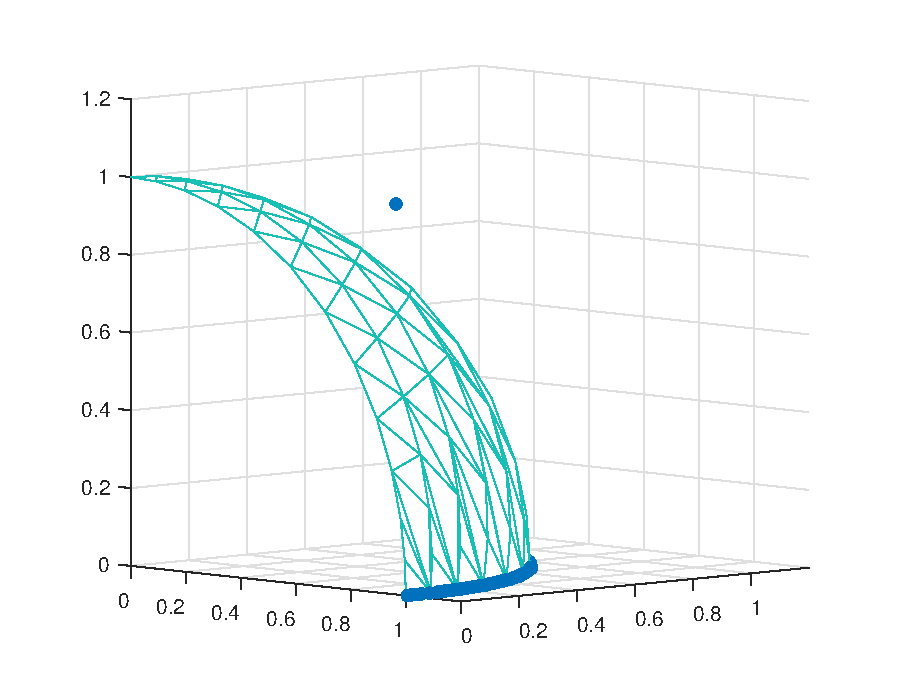
\includegraphics[height=6.45cm]{Figures/spea2_dtlz4_side.eps}\llap{\raisebox{3.1cm}{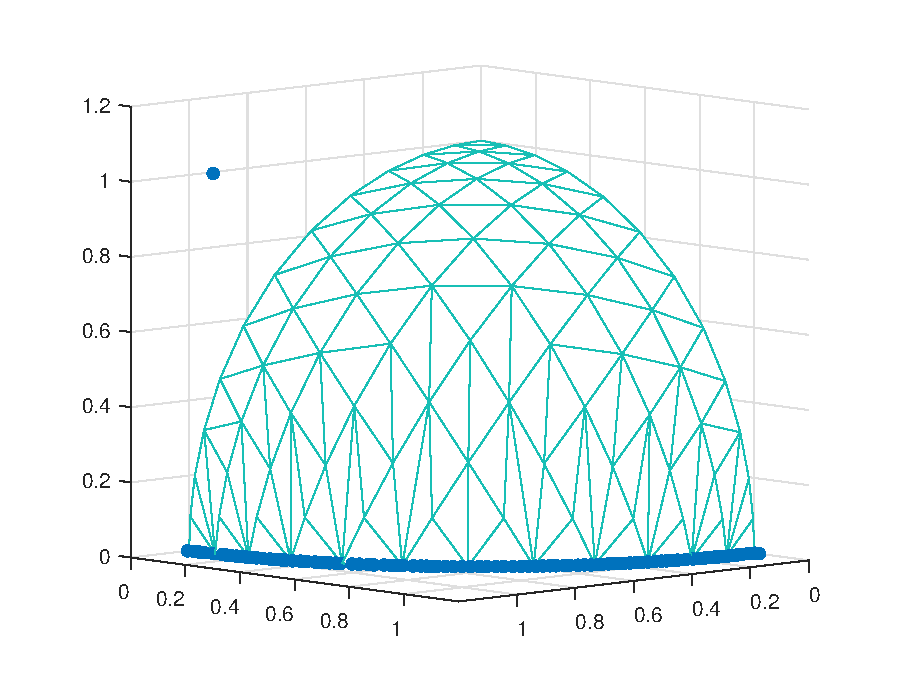
\includegraphics[height=3.1cm]{Figures/spea2_dtlz4.eps}}}
\caption{Najbolja rješenja pronađena pomoću SPEA2 na DTLZ4}
\label{fig:spea2_dtlz4}
\end{figure}

\begin{figure}[htb]
\centering
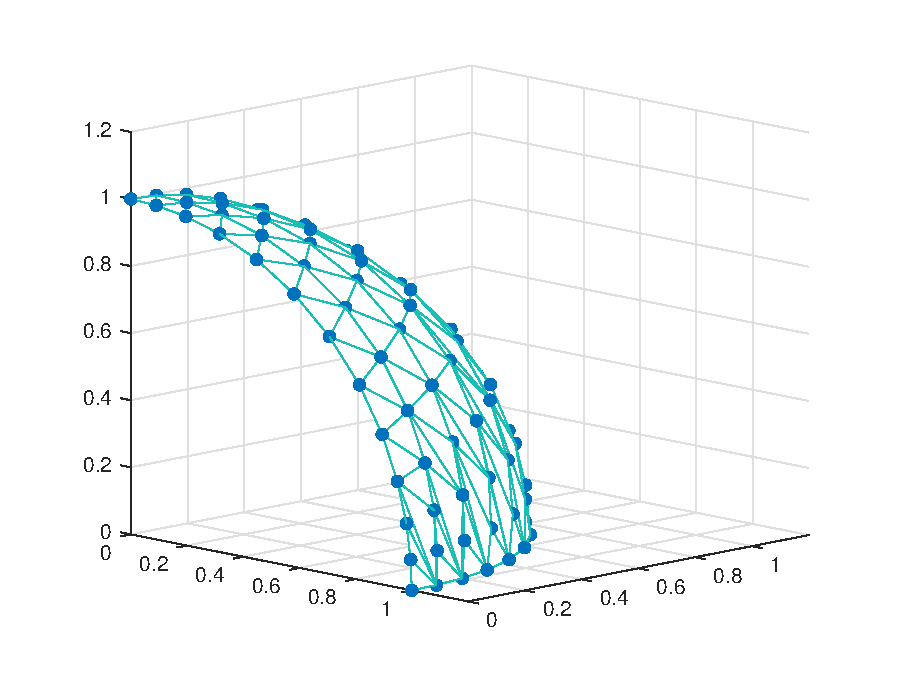
\includegraphics[height=6.45cm]{Figures/moead_pbi_dtlz4_side.eps}\llap{\raisebox{3.1cm}{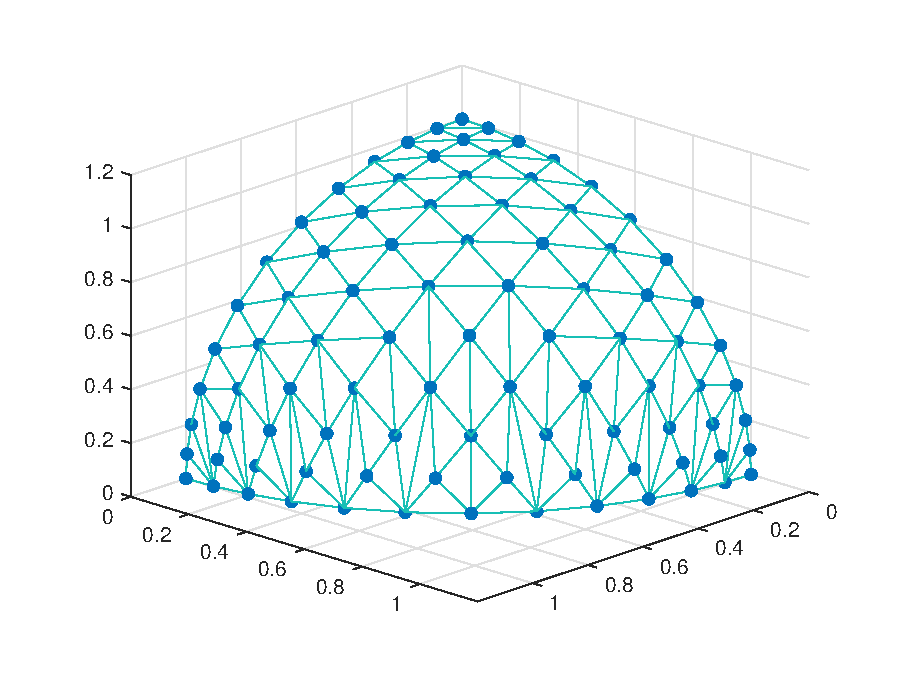
\includegraphics[height=3.1cm]{Figures/moead_pbi_dtlz4.eps}}}
\caption{Najbolja rješenja pronađena pomoću MOEA/D-PBI na DTLZ4}
\label{fig:moeadpbi_dtlz4}
\end{figure}

Od danih algoritama, samo je SPEA2 konvergirala u ravninu, no ovaj rezultat treba uzeti s oprezom jer se to isto moglo dogoditi algoritmima NSGA-II i NSGA. Naime, krajnji rezultat na ovom problemu ovisi o početnoj populaciji \citep{dtlz}. NSGA-II i NSGA, s druge strane, imaju problema s konvergencijom u globalnu Pareto frontu. Osim toga, još jednom se pokazuje superiornost algoritama NSGA-III i MOEAD-PBI nad njihovom konkurencijom u sposobnosti konvergencije i očuvanja raznovrsnosti rješenja. IGD vrijednosti algoritama za različite veličine problema DTLZ4 nalaze se u tablici \ref{tbl:dtlz4}.

\FloatBarrier
\begin{figure}[htb]
\centering
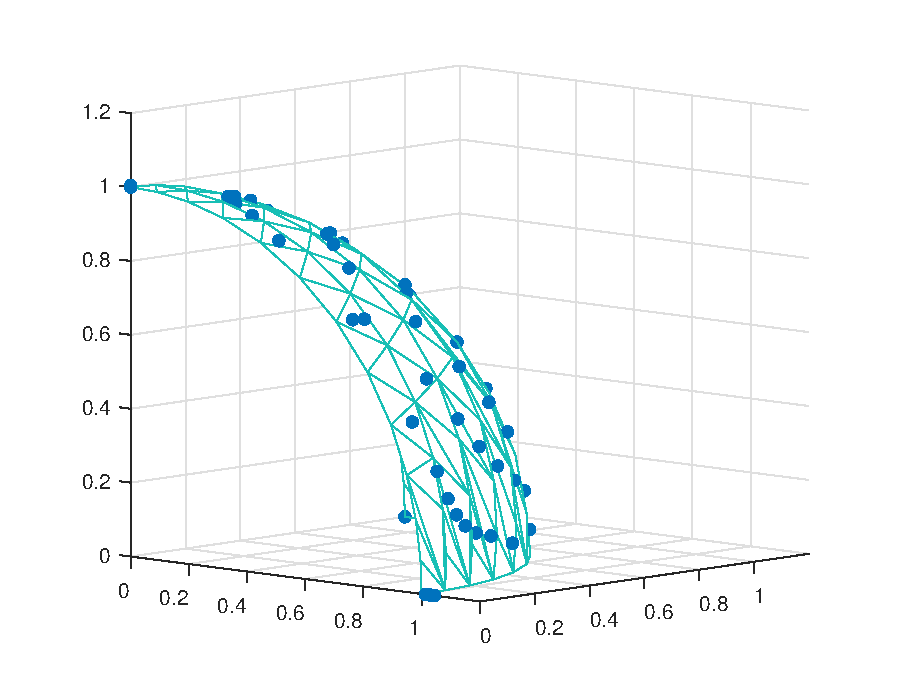
\includegraphics[height=6.45cm]{Figures/moead_tch_dtlz4_side.eps}\llap{\raisebox{3.1cm}{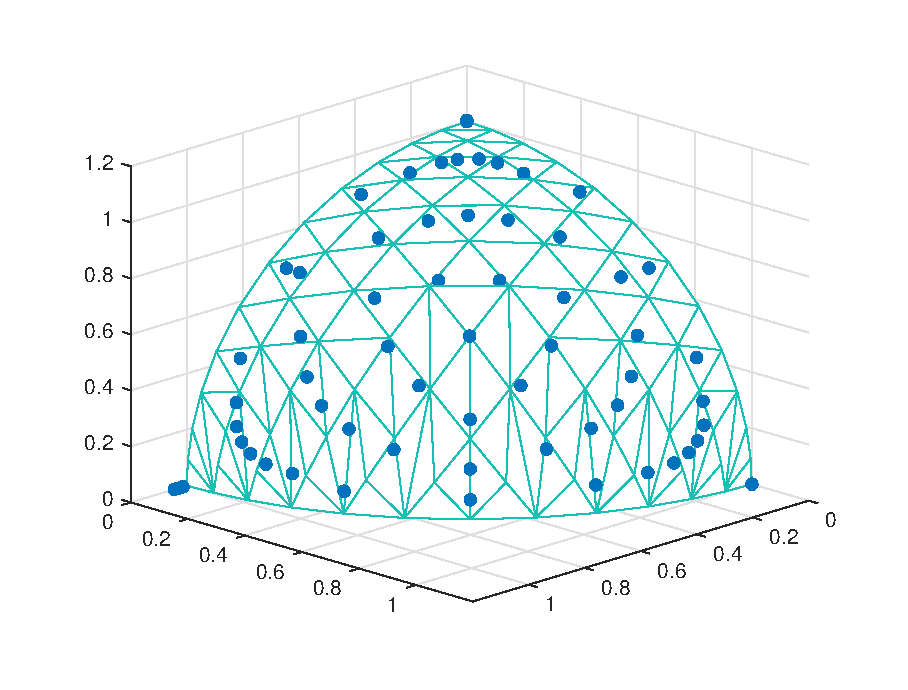
\includegraphics[height=3.1cm]{Figures/moead_tch_dtlz4.eps}}}
\caption{Najbolja rješenja pronađena pomoću MOEA/D-TCH na DTLZ4}
\label{fig:moeadtch_dtlz4}
\end{figure} 


\begin{table}[htb]
\caption{IGD vrijednosti algoritama za problem DTLZ4}
\label{tbl:dtlz4}
\centering
\small
\begin{tabular}{c|c|c|c|c|c|c} \hline
$M$ & NSGA & NSGA-II & NSGA-III & SPEA2 & MOEA/D-PBI & MOEA/D-TCH  \\ \hline
\multirow{3}{*}{2}  & $1.618\times 10^{-2}$    & $4.165\times 10^{-3}$ & $4.222\times 10^{-4}$ & $4.093\times 10^{-3}$ & $\mathbf{1.616\times 10^{-4}}$ & $2.576\times 10^{-4}$\\
			        & $2.508\times 10^{-2}$    & $5.075\times 10^{-3}$ & $\mathbf{1.046\times 10^{-3}}$ & $7.417\times 10^{-1}$ & $7.417\times 10^{-1}$ & $8.555\times 10^{-3}$\\
                    & $7.417\times 10^{-1}$    & $7.417\times 10^{-1}$ & $7.417\times 10^{-1}$ & $7.417\times 10^{-1}$ & $7.417\times 10^{-1}$ & $7.417\times 10^{-1}$\\ \hline
\multirow{3}{*}{3}  & $1.022\times 10^{-1}$    & $6.944\times 10^{-2}$ & $1.818\times 10^{-3}$ & $4.205\times 10^{-1}$ & $\mathbf{2.399\times 10^{-4}}$ & $7.934\times 10^{-2}$\\
			        & $5.369\times 10^{-1}$    & $4.103\times 10^{-1}$ & $\mathbf{3.114\times 10^{-3}}$ & $5.317\times 10^{-1}$ & $2.682\times 10^{-1}$ & $5.321\times 10^{-1}$\\
                    & $9.503\times 10^{-1}$    & $9.503\times 10^{-1}$ & $9.503\times 10^{-1}$ & $9.503\times 10^{-1}$ & $9.503\times 10^{-1}$ & $9.503\times 10^{-1}$\\ \hline
\multirow{3}{*}{5}  & $2.630\times 10^{-1}$    & $2.252\times 10^{-1}$ & $\mathbf{3.871\times 10^{-3}}$ & $6.176\times 10^{-1}$ & $1.120\times 10^{-2}$ & $5.098\times 10^{-1}$\\
			        & $4.517\times 10^{-1}$    & $4.540\times 10^{-1}$ & $\mathbf{5.252\times 10^{-3}}$ & $7.867\times 10^{-1}$ & $2.310\times 10^{-1}$ & $6.690\times 10^{-1}$\\
                    & $8.716\times 10^{-1}$    & $7.064\times 10^{-1}$ & $\mathbf{6.875\times 10^{-3}}$ & $8.697\times 10^{-1}$ & $6.205\times 10^{-1}$ & $8.748\times 10^{-1}$\\ \hline
\multirow{3}{*}{8}  & $1.069$                  & $8.542\times 10^{-1}$ & $\mathbf{8.555\times 10^{-3}}$ & $7.500\times 10^{-1}$ & $2.355\times 10^{-1}$ & $6.483\times 10^{-1}$\\
			        & $1.079$                  & $1.308$               & $\mathbf{1.189\times 10^{-2}}$ & $9.848\times 10^{-1}$ & $5.817\times 10^{-1}$ & $7.744\times 10^{-1}$\\
                    & $1.229$                  & $1.665$               & $\mathbf{1.391\times 10^{-2}}$ & $1.065$               & $7.458\times 10^{-1}$ & $9.140\times 10^{-1}$\\ \hline
\multirow{3}{*}{10} & $1.734$                  & $1.371$               & $\mathbf{1.290\times 10^{-2}}$ & $8.795\times 10^{-1}$ & $4.740\times 10^{-2}$ & $6.133\times 10^{-1}$\\
			        & $1.832$                  & $1.516$               & $\mathbf{1.375\times 10^{-2}}$ & $9.844\times 10^{-1}$ & $3.723\times 10^{-1}$ & $7.832\times 10^{-1}$\\
                    & $1.920$                  & $1.685$               & $\mathbf{1.565\times 10^{-2}}$ & $1.041$               & $6.248\times 10^{-1}$ & $8.845\times 10^{-1}$\\ \hline\end{tabular}
\end{table}
Za algoritme NSGA, NSGA-II, SPEA2 i MOEA/D-TCH vrijedi da, kada veličina problema prijeđe 3 ciljne funkcije, na ovom problemu daju lošu IGD vrijednost. Iz ovog se da zaključiti da ako se poveća broj ciljnih funkcija, ti algoritmi neće više biti u stanju prilagoditi svoj postupak očuvanja raznovrsnosti. Osim toga, vidimo iz tablice da NSGA-III daje najbolje rezultate, dok skup rješenja pronađen pomoću MOEA/D-PBI propada u kvaliteti ako se poveća broj ciljnih funkcija. 

\chapter{Zaključak}
Nakon što smo ukratko opisali problem višekriterijske optimizacije, naveli i opisali neke od algoritama kojima se on rješava te ispitali njihov rad, ponovimo najbitnije rezultate:
\begin{itemize}
\item NSGA-III i MOEA/D-PBI pokazuju najbolje rezultate na svim ispitnim primjerima,
\item za dane probleme, NSGA konzistentno daje najgora rješenja,
\item za ponuđene probleme sa sfernom Pareto frontom, NSGA-III pronalazi bolja rješenja od MOEA/D-PBI,
\item povećanjem broja ciljnih funkcija algoritmima NSGA, NSGA-II, SPEA2 i \text{MOEA/D-TCH} znatno se pogoršava izvedba,
\item MOEA/D-PBI se ispostavlja kao bolji pristup od MOEA/D-TCH.
\end{itemize}  
Međutim, treba napomenuti neke od nedostataka NSGA-III i MOEA/D-PBI. Oba algoritma u sebi sadrže vrlo snažne pretpostavke o obliku Pareto fronte, konkretno da su rješenja dobro rasprostranjena na Pareto fronti te da je gustoća rješenja na pojedinim dijelovima slična gustoći rasporeda referentnih točaka, odnosno vektora težina. Nedavni rad \citet{problem} pokazao je da se rezultati ovih algoritama na DTLZ setu znatno pogoršavaju kad se umjesto minimizacije provodi maksimizacija ciljnih funkcija pomnoženih faktorom $-1$, kako je navedeno u odjeljku \ref{sec:kriterij}, iako se očekuje da za takvu formulaciju problema neće biti promjene u rezultatima koje algoritmi postižu. NSGA-III nastoji riješiti takav problem omogućujući korisniku da sam unese svoje referentne točke, ali pri višekriterijskoj optimizaciji u stvarnom svijetu, rijetko znamo dobru aproksimaciju Pareto fronte. Sve navedeno upućuje na potrebu nastavka istraživanja u području višekriterijske optimizacije, pogotovo problema s većim brojem ciljnih funkcija, da bi se pronašli fleksibilniji algoritmi.

\bibliography{literatura}
\bibliographystyle{fer}

\begin{sazetak}
U ovom radu opisuje se problem višekriterijske optimizacije, definiraju kriteriji za usporedbu rješenja te izlažu algoritmi za višekriterijsku optimizaciju: NSGA, NSGA-II, NSGA-III, SPEA2, MOEA/D-PBI i MOEA/D-TCH. Algoritmi su ispitani na problemima DTLZ1, DTLZ2, DTLZ3 i DTLZ4 koji od 2 do 10 ciljnih funkcija te su njihovi rezultati međusobno uspoređeni. NSGA-III i MOEA/D-PBI su polučili najbolje rezultate na problemima s više od 5 ciljnih funkcija, dok su se ostali algoritmi pokazali gotovo neupotrebljivima. Za probleme s manje od 5 ciljnih funkcija svi su algoritmi pronašli prihvatljiv skup rješenja.

\kljucnerijeci{Pareto fronta, ciljna funkcija, algoritam, DTLZ, IGD}
\end{sazetak}

% TODO: Navedite naslov na engleskom jeziku.
\engtitle{Algorithms for multiobjective and many-objective optimization}
\begin{abstract}
In this paper, the multiobjective optimization problem is described, as well as the criteria for the comparison of different solutions. Multiobjective optimization algorithms are presented: NSGA, NSGA-II, NSGA-III, SPEA2, MOEA/D-PBI and MOEA/D-TCH. The algorithms are tested on 2-to-10-objective DTLZ1, DTLZ2, DTLZ3 and DTLZ4 problems and their performance is compared. NSGA-III and MOEA/D-PBI had the best results on problems with more than 5 objective functions, whereas other algorithms have performed poorly. On problems with less than 5 objective functions, all algorithms have found an acceptable set of solutions.

\keywords{Pareto front, objective function, algorithm, DTLZ, IGD}
\end{abstract}

\end{document}
